%=============================================================================
%  Drishti-AI — full paper (normal single-column article format, 12pt)
%  Compiles on Overleaf with pdfLaTeX. Bibliography is embedded (no BibTeX
%  run needed). Upload the /figures folder alongside this file.
%=============================================================================
\documentclass[12pt]{article}

\usepackage[utf8]{inputenc}
\usepackage[T1]{fontenc}
\usepackage[margin=1in]{geometry}
\usepackage{graphicx}
\usepackage{booktabs}
\usepackage{array}
\usepackage{amsmath,amssymb}
\usepackage{float}
\usepackage{caption}
\usepackage{microtype}
\usepackage{url}
\usepackage[hidelinks]{hyperref}

\captionsetup{font=small,labelfont=bf}
\graphicspath{{./}{figures/}}
\setlength{\parskip}{4pt}
\renewcommand{\arraystretch}{1.15}

\title{\textbf{Drishti-AI: An Offline, Edge-Deployable Multi-Module AI Platform\\
for Quality, Maintenance, and Demand Intelligence in\\ MSME Manufacturing}}
\author{L.~Yashwanth Reddy \\
  \small School of Computer Science and Engineering \\
  \small (Artificial Intelligence and Machine Learning) \\
  \small SRM Institute of Science and Technology, Ramapuram \\
  \small Chennai, Tamil Nadu, India \\
  \small \texttt{nadhahari44@gmail.com}}
\date{\today}

\begin{document}
\maketitle

\begin{abstract}
\noindent
Most of India's factories are small shops, yet the machine-learning tools that
cut defects, downtime, and excess stock assume things those shops rarely have:
cloud servers, GPUs, and staff who read English. \textbf{Drishti-AI} is built for
the shop that has none of them. Four parts run on an ordinary CPU with no network
and report to one dashboard --- a camera defect check, a Hindi alert that tells
the operator what to do next, a tool-wear predictor from vibration and current
signals, and a weekly demand forecast. We trained and tested each part on public
data and kept the test strict: separate held-out sets, model choices made on
validation and never on the test set, comparisons against plain baselines, and
three random seeds for the vision model. The defect model, a MobileNetV2 with
2.23~million parameters, scores $99.39\% \pm 0.24$ on the test set, ties a
ResNet-50 ten times its size, and reads an image in 2.37~ms on a CPU through
ONNX. The maintenance model reaches $R^2 = 0.545$ on tools it never saw in
training, and the forecaster lands at 19.7\% weighted absolute percentage error
(WAPE), ahead of naïve, seasonal, and Prophet baselines. Each result comes with
its limits. We offer the system as a reproducible proof of concept, not a
finished product.
\end{abstract}

\textbf{Keywords:} edge AI, defect detection, predictive maintenance, demand
forecasting, MobileNetV2, XGBoost, MSME manufacturing, offline inference.

%=============================================================================
\section{Introduction}

Small and mid-sized manufacturers employ much of India's industrial workforce and
turn out a large share of its goods, usually on thin margins and patchy internet.
The AI products that promise fewer defects, less downtime, and smarter stock are
aimed elsewhere --- at plants with cloud accounts, GPU servers, and dashboards
written in English. A shop that casts or machines a few thousand parts a month has
none of that, so the gains from modern machine learning mostly pass it by.

Four problems keep turning up on these floors. Quality checks are done by eye, so
defects reach the customer. Tools wear down and stop a machine with no warning.
Stock gets ordered on a hunch, which locks up cash in the wrong parts. And running
under all three is a language gap: the person who has to act on a warning often
cannot read the English a model prints.

Drishti-AI takes on the four together. It is one platform of four parts that share
a single data format and one dashboard, yet stay loosely joined, so a shop can
start with one part and add the rest later. Every part runs on ordinary hardware
without a network, and the alert layer speaks the operator's language. We are not
claiming a product that ships tomorrow. The aim is narrower, and more useful for
it: to show plainly, and in a way anyone can repeat, that each part works on public
data under a fair test, and that the four fit into one affordable design.

Here is what the paper adds, worked out in the sections that follow:
\begin{itemize}
  \item A four-part system for small manufacturers that runs offline and shares one
        JSON format (Section~\ref{sec:arch}).
  \item A defect detector small enough for the edge --- 2.23~M parameters, 2.37~ms
        per image --- that ties ResNet-50 within seed noise (Section~\ref{sec:res-m1}).
  \item A tool-life test built around a by-tool split, so the score reflects tools
        the model never saw (Section~\ref{sec:res-m3}).
  \item A demand forecaster with honest prediction intervals that beats naïve,
        seasonal, and Prophet baselines (Section~\ref{sec:res-m4}).
  \item A Hindi alert layer that turns a model's verdict into something the
        operator can act on (Section~\ref{sec:methods}).
\end{itemize}

%=============================================================================
\section{Related Work}

\paragraph{Visual defect detection.}
Convolutional networks have become the usual choice for automated surface
inspection, used to both segment and classify defects across many industries [44].
For a model that must run on cheap hardware, the backbone matters. MobileNetV2 [1]
uses inverted residuals and linear bottlenecks to cut parameters and latency at
little cost to accuracy, unlike heavier residual nets [3] or scaled families such
as EfficientNet [10]. We chose MobileNetV2 for that reason, then checked that on
castings it gives up nothing measurable to the larger network.

\paragraph{Predictive maintenance and remaining useful life.}
Data-driven prognostics estimate how much life a machine has left from its
condition signals; reviews map the whole path from raw signal to a life estimate
[45] and cover deep-learning takes on machine health [46]. Gradient-boosted trees
[11], [12] fit the tabular statistics common here well and cost little to run. One
trap shows up again and again --- testing on rows from tools the model has already
partly seen --- and a strict by-tool split avoids it. That is the split we use.

\paragraph{Demand forecasting.}
Old and new forecasters sit side by side in practice. Prophet [31] handles
seasonality with little tuning, while the M4 [34] and M5 [36] competitions showed
that boosted trees on lag and calendar features hold their own against far more
complex methods. Scale-free error measures like WAPE suit demand that is spiky and
spread across many series [35], and quantile regression [32] gives prediction
intervals with real coverage. We put these together: an XGBoost point model with a
pair of quantile models, scored by WAPE.

\paragraph{Transfer learning, explainability, and edge deployment.}
Starting from an ImageNet-pretrained backbone is standard [16], [17], and it is
where our vision model begins. Grad-CAM [18] shows which pixels drove a prediction,
which helps a user trust the output. Running models on small devices is helped by
compact backbones [2], quantization [28], and distillation [29], and by the wider
effort to fit models onto microcontrollers and edge CPUs [30]. Making an alert
readable to someone who does not work in English ties into low-resource Indic
NLP [48].

%=============================================================================
\section{System Overview and Architecture}
\label{sec:arch}

Drishti-AI has four parts that take shop-floor inputs and meet at one dashboard
(Figure~\ref{fig:arch}). Module~1 checks part images for defects; its verdict goes
to Module~2, which writes a short Hindi message and a suggested fix for the
operator. Module~3 reads vibration and current signals to judge tool wear, and
Module~4 reads past orders to forecast next week's demand. All four write to the
same JSON format, so the dashboard can show quality, uptime, and stock in one place
for the owner.

Two decisions shape the design. The parts talk only through the shared format, so
a shop can run one of them and bolt on the others later with no rework. And
everything runs on a plain CPU without a network: the models are small, and the
vision model is exported to ONNX [22], [23] for quick inference with few
dependencies. Nothing needs the cloud at run time, which fits a floor with spotty
connectivity and keeps the running cost close to nothing.

\begin{figure}[H]
\centering
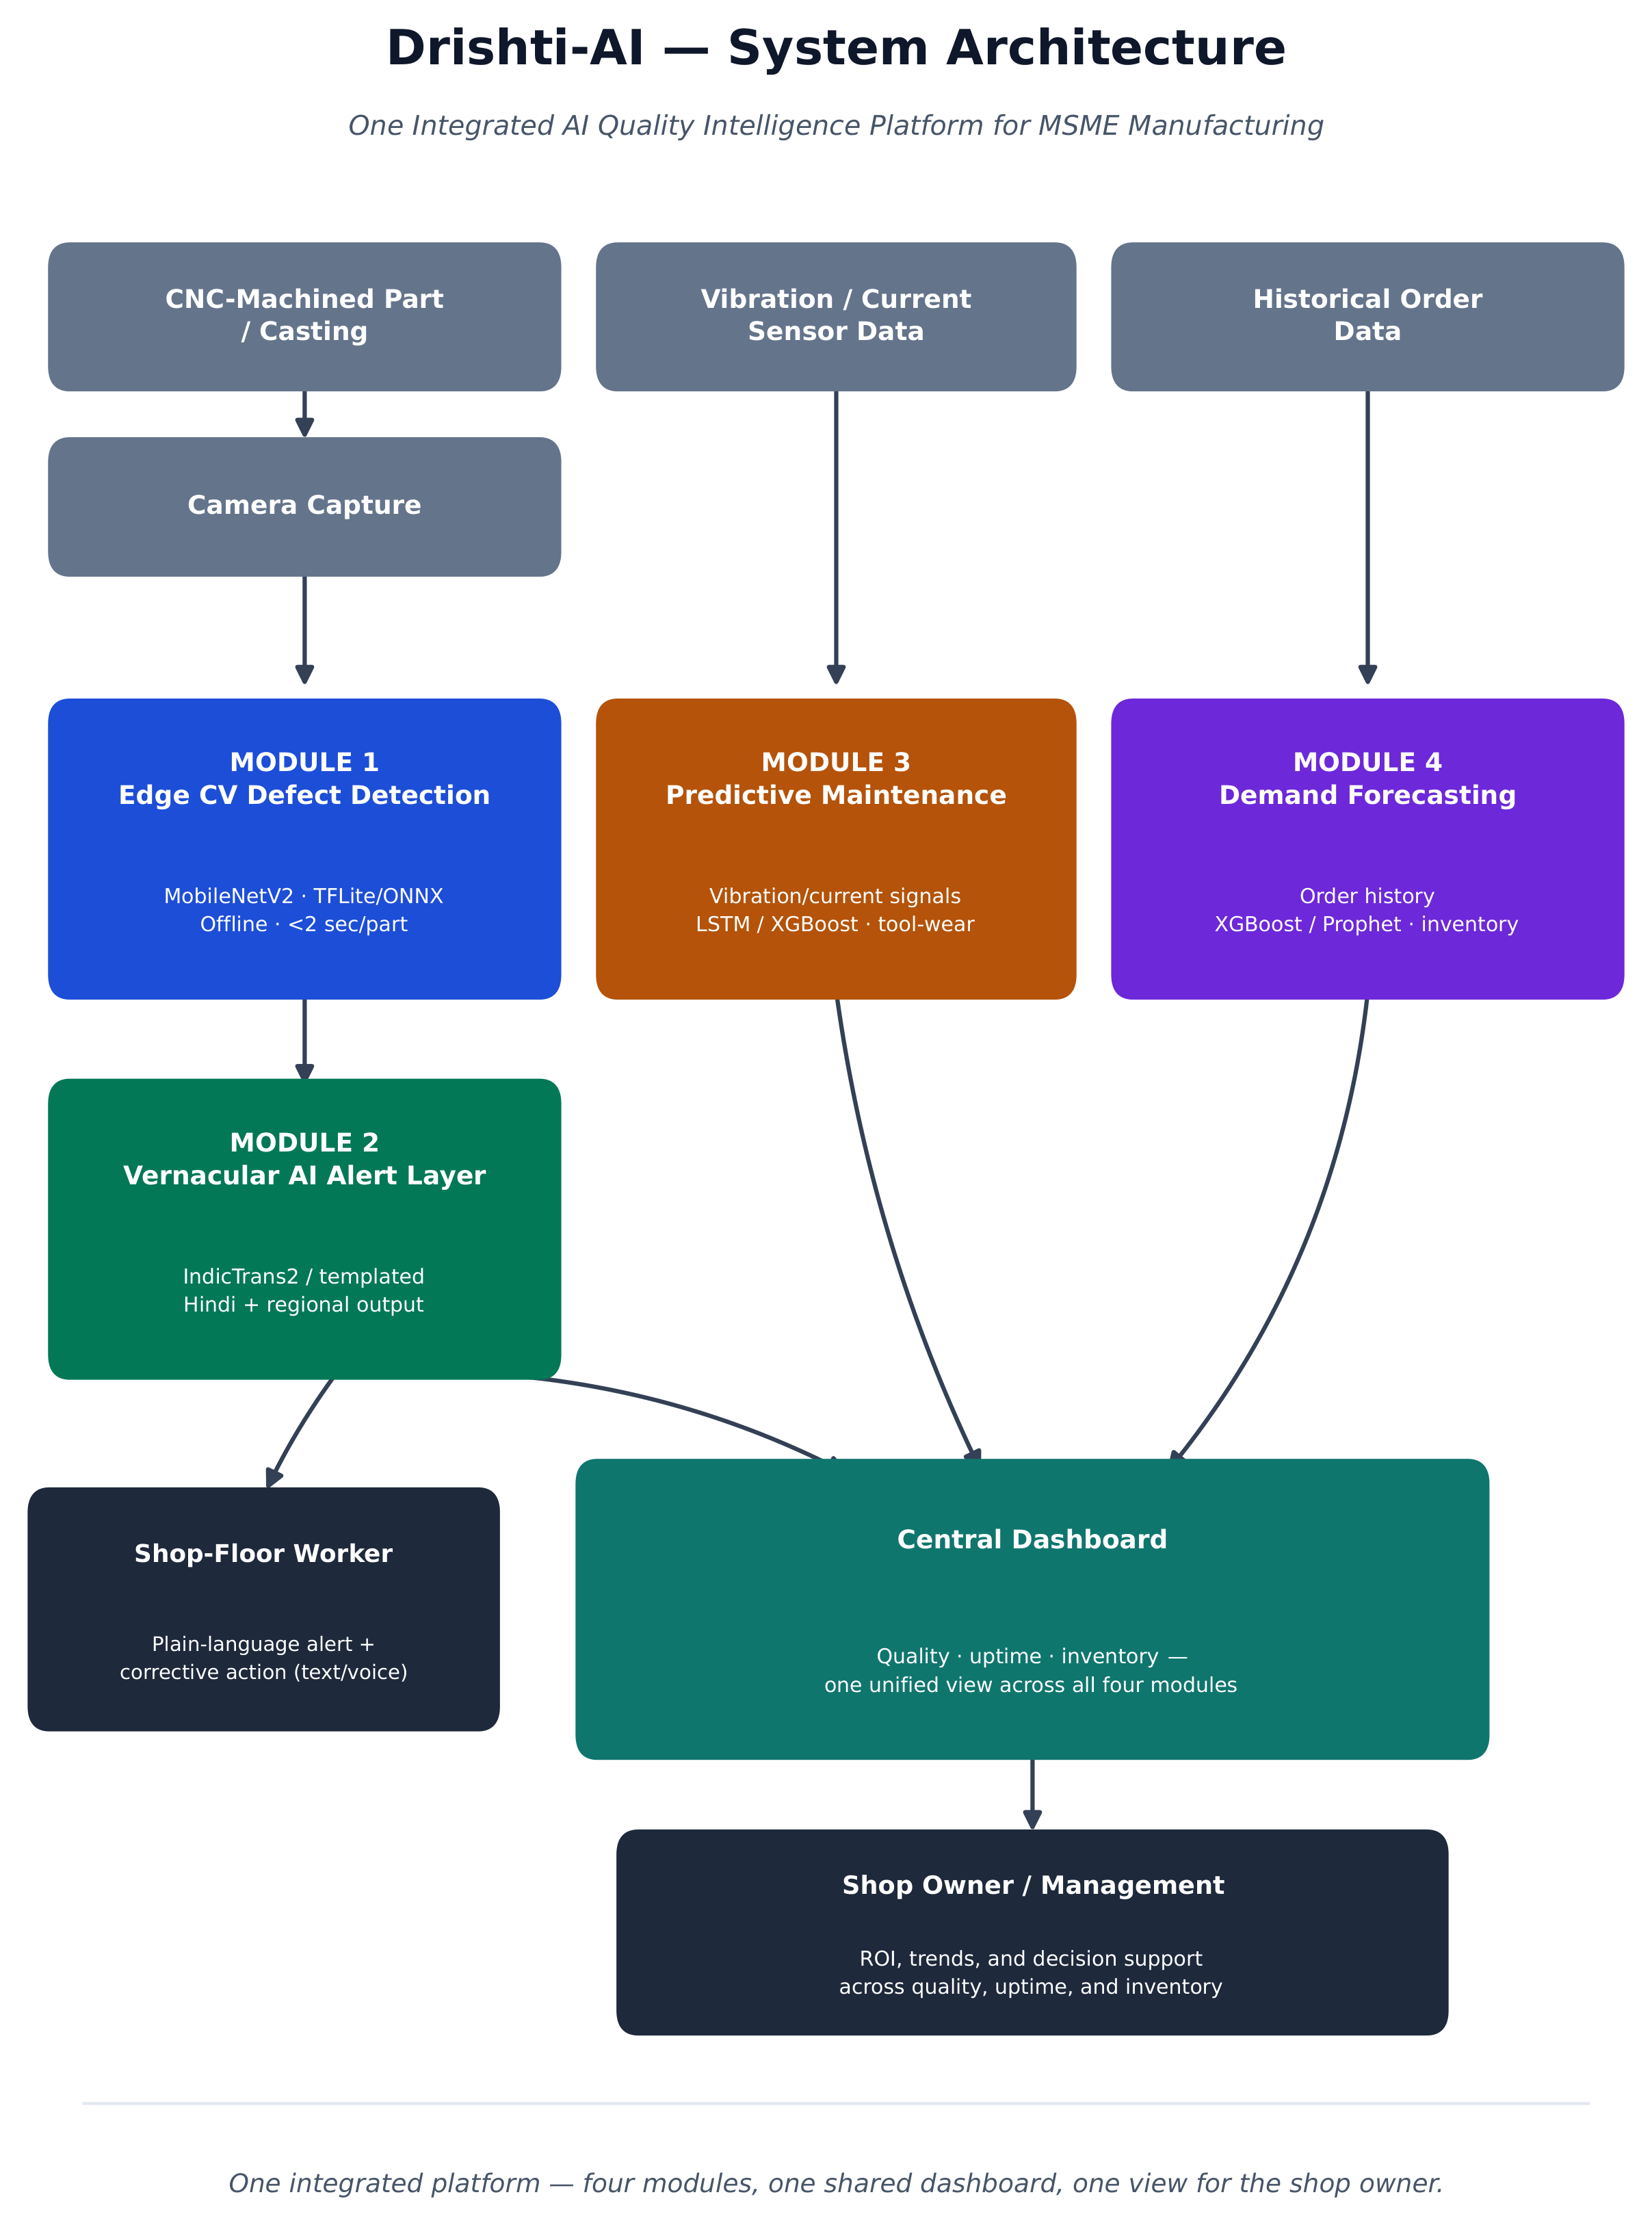
\includegraphics[width=0.72\textwidth]{fig01_architecture_author.png}
\caption{Drishti-AI system architecture: four decoupled modules feed a shared
central dashboard and run fully offline on commodity edge hardware. Module~1
(vision) triggers the Module~2 vernacular alert to the worker; Modules~3 and~4
feed uptime and inventory intelligence to management.}
\label{fig:arch}
\end{figure}

Table~\ref{tab:overview} lays out the four modules with their models, data, and
headline numbers. These come from public datasets under held-out tests, not from a
running factory.

\begin{table}[H]
\caption{System overview: one row per module.}
\label{tab:overview}
\centering
\small
\begin{tabular}{@{}p{0.7cm}p{3.4cm}p{2.9cm}p{2.9cm}p{2.7cm}@{}}
\toprule
Mod. & Task & Model & Dataset & Headline result \\
\midrule
M1 & Casting surface-defect classification & MobileNetV2 (transfer) & Casting images [41] & $99.39\%\pm0.24$ test acc.; 2.37~ms/img \\
M2 & Vernacular (Hindi) operator alert & Rule-mapped template NLG & Derived from M1 & Deterministic Hindi alert per inspection \\
M3 & Remaining useful life of CNC tools & XGBoost regressor & CNC milling [42] & $R^2=0.545$ on unseen tools \\
M4 & Weekly demand forecast per category & XGBoost + quantile pair & Product demand [43] & 19.7\% WAPE; P10--P90 intervals \\
\bottomrule
\end{tabular}
\end{table}

%=============================================================================
\section{Datasets}
\label{sec:data}

Each learning module uses one public dataset (Table~\ref{tab:datasets}).
\textbf{Module~1} uses a set of casting inspection photos [41] of submersible-pump
impellers, each marked defective (\texttt{def\_front}) or acceptable
(\texttt{ok\_front}). We train on 6{,}633 images and set aside a fixed test set of
715 (453 defective, 262 acceptable); Figure~\ref{fig:datasets} (left) shows the
split.

\textbf{Module~3} uses a CNC milling dataset [42]: 968 cutting passes from 14
physical tools, each followed from new to worn out. Every pass comes with
time-domain statistics --- minimum, maximum, mean, standard deviation, skewness,
kurtosis --- over the spindle and axis accelerometers and the three-phase currents,
plus a little tool metadata, and a label giving normalized cycles to failure (1.0
new, 0.0 failed).

\textbf{Module~4} uses a product-demand dataset [43] of about 1.05~million order
lines across 2{,}160 products in four warehouses. We roll the orders up to weekly
totals per category and keep the 28 categories with enough history.
Figure~\ref{fig:datasets} (right) shows how far category volumes spread --- from
millions of units a week down to tens --- which is why some categories are much
harder to forecast than others.

\begin{table}[H]
\caption{Datasets used, one per learning module.}
\label{tab:datasets}
\centering
\small
\begin{tabular}{@{}p{2.4cm}p{0.8cm}p{3.2cm}p{2.4cm}p{3.2cm}@{}}
\toprule
Dataset & Mod. & Size & Domain & Split protocol \\
\midrule
Casting images [41] & M1 & $\sim$7.3k images (300$\times$300) & Impeller surface & Stratified train/val (0.15); fixed test $n{=}715$ \\
CNC milling [42] & M3 & 968 passes, 14 tools & Vibration + current & By-tool split: 9 train / 4 test; tool~11 dropped \\
Product demand [43] & M4 & 1{,}048{,}575 orders $\to$ 28 categories & Multi-warehouse orders & Temporal cut-off 2016-01-11; 52 held-out weeks \\
\bottomrule
\end{tabular}
\end{table}

\begin{figure}[H]
\centering
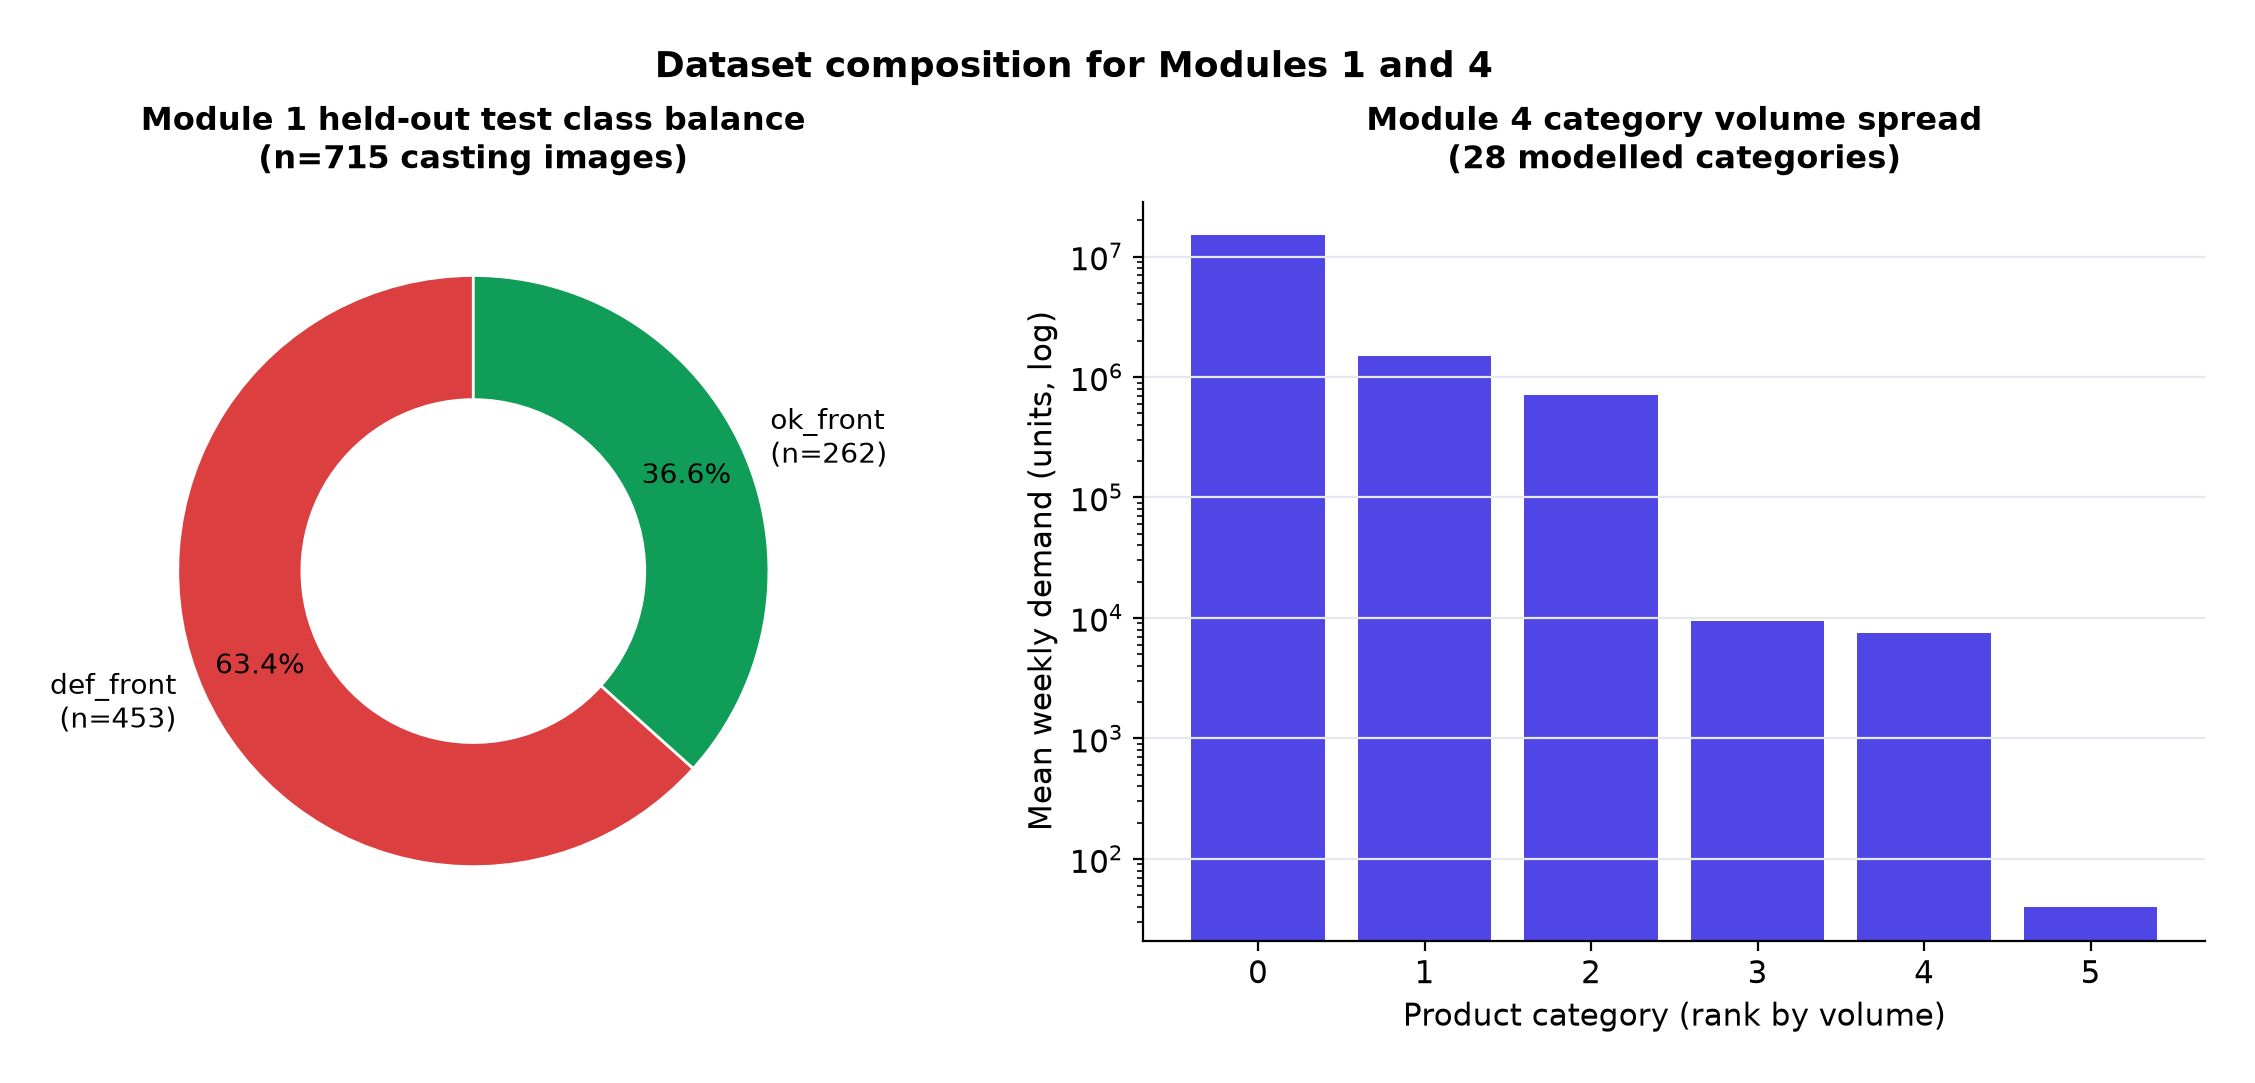
\includegraphics[width=\textwidth]{fig14_dataset_overview.png}
\caption{Dataset composition. Left: the Module~1 held-out test set ($n=715$) is
mildly imbalanced (63\% defective, 37\% acceptable), which is why we report
macro-F1 alongside accuracy so the smaller class is not masked. Right: Module~4
mean weekly demand per category on a logarithmic axis; volumes span more than
five orders of magnitude, so a scale-free error (WAPE) is essential and the
lowest-volume categories are inherently the hardest to forecast.}
\label{fig:datasets}
\end{figure}

%=============================================================================
\section{Methods}
\label{sec:methods}

\subsection{Module 1 --- Defect detection}

Module~1 is an image classifier that starts from a MobileNetV2 backbone [1]
pretrained on ImageNet [4]. We swap in a new head and train in two stages: 15 epochs
with the backbone frozen (Adam [9], learning rate $10^{-3}$), then 5 more with the
top 20 backbone layers unfrozen at $10^{-5}$. Images go in at $224\times224$, 32 at
a time. The part that matters most is the split. We hold out 15\% of the training
folder as a stratified validation set, pick the model on validation accuracy, and
touch the test set only once --- that keeps the test score honest. We run the whole
thing three times, with seeds 1, 2, and 42, to see how much the result moves.
Table~\ref{tab:m1cfg} has the settings. To see what the model looks at, we use
Grad-CAM [18].

\begin{table}[H]
\caption{Module~1 training configuration.}
\label{tab:m1cfg}
\centering
\small
\begin{tabular}{@{}p{5.2cm}p{7.2cm}@{}}
\toprule
Hyperparameter & Value \\
\midrule
Backbone / initialization & MobileNetV2, ImageNet-pretrained \\
Head schedule & 15 epochs, Adam, lr $10^{-3}$ (backbone frozen) \\
Fine-tune schedule & 5 epochs, Adam, lr $10^{-5}$, top 20 layers unfrozen \\
Batch size / image size & 32 / $224\times224$ \\
Validation split & 15\%, stratified (test set untouched) \\
Model selection & best validation accuracy; test scored once \\
Random seeds & 1, 2, 42 \\
\bottomrule
\end{tabular}
\end{table}

\subsection{Module 2 --- Vernacular alert}

Module~2 turns a Module~1 verdict into a short Hindi message with a suggested fix.
Instead of a full translation model, we fill a fixed Hindi template with the class,
the confidence, and the part number. That is a deliberate choice for an offline
shop: it is fast, needs no GPU, and produces text you can read and check. If richer
wording is wanted later, a neural Indic translator [48] can drop in.

\subsection{Module 3 --- Predictive maintenance}

Module~3 predicts a tool's normalized remaining life from the per-pass statistics
with an XGBoost regressor [11], a boosted-tree model [12] that fits tabular sensor
data well. The split is the thing to get right. Consecutive passes of one tool trace
a single wear curve, so a random row split would let the model fill in gaps on tools
it has already seen and look better than it is. We split by tool instead --- nine
tools to train on, four held out completely --- and drop a tool with only one
recorded cycle. Tables~\ref{tab:m3data} and~\ref{tab:m3cfg} give the data and the
settings.

\begin{table}[H]
\caption{Module~3 data and by-tool split.}
\label{tab:m3data}
\centering
\small
\begin{tabular}{@{}p{4.0cm}p{8.4cm}@{}}
\toprule
Item & Value \\
\midrule
Target & Normalized cycles-to-failure (1.0 fresh $\to$ 0.0 failure) \\
Features & 130 time-domain statistics per sensor channel + tool metadata \\
Sensors & Spindle/axis accelerometers; three-phase spindle/axis currents \\
Train tools (9) & 3, 4, 5, 6, 7, 8, 9, 102, 105 \\
Test tools (4, held out) & 2, 10, 101, 103 \\
Dropped & Tool 11 (single recorded cycle) \\
\bottomrule
\end{tabular}
\end{table}

\begin{table}[H]
\caption{Module~3 training configuration.}
\label{tab:m3cfg}
\centering
\small
\begin{tabular}{@{}p{5.4cm}p{7.0cm}@{}}
\toprule
Hyperparameter & Value \\
\midrule
Estimator & XGBoost regressor \\
Number of trees / max depth & 300 / 4 \\
Learning rate & 0.05 \\
Subsample / column subsample & 0.8 / 0.8 \\
Split & Grouped shuffle by tool, 25\% held out, seed 42 \\
\bottomrule
\end{tabular}
\end{table}

\subsection{Module 4 --- Demand forecasting}

Module~4 forecasts next week's demand per category with an XGBoost regressor [11]
on 18 features (Table~\ref{tab:m4feat}): lags at 1, 2, 3, 4, 8, 12, and 52 weeks,
rolling means and standard deviations, an exponentially weighted mean, two short
trend terms, and cyclic calendar encodings. We left the category identifier out on
purpose --- an ablation showed it made the held-out error worse, because it pushed
the model to memorize each category's level instead of learning patterns that carry
across categories. For uncertainty we train a matched pair of quantile models
($\alpha = 0.1$ and $0.9$) [32], which gives an 80\% P10--P90 band around each
forecast. The point model uses a fixed 300 trees; early stopping was less stable on
this data.

\begin{table}[H]
\caption{Module~4 feature set (18 features).}
\label{tab:m4feat}
\centering
\small
\begin{tabular}{@{}p{3.0cm}p{9.4cm}@{}}
\toprule
Group & Features \\
\midrule
Lags & \texttt{lag\_1, lag\_2, lag\_3, lag\_4, lag\_8, lag\_12, lag\_52} \\
Rolling / smoothing & \texttt{rolling\_mean\_4/8/13}, \texttt{rolling\_std\_4}, \texttt{ewma\_4} \\
Trend & \texttt{trend\_1}, \texttt{trend\_4} \\
Calendar & \texttt{month}, \texttt{weekofyear}, \texttt{woy\_sin}, \texttt{woy\_cos} \\
\bottomrule
\end{tabular}
\end{table}

%=============================================================================
\section{Experimental Setup}
\label{sec:setup}

Each module is scored with metrics that fit its job (Table~\ref{tab:metrics}).
Module~1 uses accuracy and macro-F1, and we watch the false negatives --- defective
parts called acceptable --- since that is the error that hurts. Module~3 uses RMSE,
MAE, and $R^2$. Module~4 uses WAPE,
$\text{WAPE} = \sum_t |y_t - \hat{y}_t| \big/ \sum_t |y_t|$, a scale-free error that
makes sense when series differ by orders of magnitude, together with how often the
true value lands inside the P10--P90 band.

Every comparison carries plain baselines, so a gain means something instead of
hanging in the air: a constant-mean and a linear model for maintenance, and naïve,
seasonal-naïve, and Prophet forecasters for demand. Single runs can fool you, so the
vision architectures run over three seeds and we report the mean and standard
deviation. The software (Table~\ref{tab:env}) is all open source and pinned, and the
seeds and commands ship with the code.

\begin{table}[H]
\caption{Evaluation metrics.}
\label{tab:metrics}
\centering
\small
\begin{tabular}{@{}p{2.8cm}p{7.0cm}p{2.0cm}@{}}
\toprule
Metric & Definition & Used in \\
\midrule
Accuracy / Macro-F1 & Standard classification measures & M1 \\
False negatives & True-defect predicted acceptable (safety-critical) & M1 \\
RMSE / MAE / $R^2$ & Regression error and explained variance & M3 \\
WAPE & $\sum|y-\hat{y}| / \sum|y|$ (scale-free) & M4 \\
Interval coverage & Fraction of actuals inside P10--P90 & M4 \\
\bottomrule
\end{tabular}
\end{table}

\begin{table}[H]
\caption{Software and environment.}
\label{tab:env}
\centering
\small
\begin{tabular}{@{}p{4.2cm}p{8.0cm}@{}}
\toprule
Component & Version / setting \\
\midrule
Deep learning & PyTorch [21]; export via ONNX / ONNX Runtime [22], [23] \\
Gradient boosting & XGBoost [11] \\
Classic ML / arrays & scikit-learn [24], NumPy [25], pandas [26] \\
Forecasting baseline & Prophet [31] \\
Plotting & Matplotlib [27] \\
Random seeds & $\{1,2,42\}$ (M1 architectures); 42 (M3, M4) \\
\bottomrule
\end{tabular}
\end{table}

%=============================================================================
\section{Results}

\subsection{Module 1 --- Defect detection}
\label{sec:res-m1}

Table~\ref{tab:m1arch} puts three architectures on the same split. Our MobileNetV2
hits $99.39\% \pm 0.24$ with 2.23~million parameters --- close enough to a ResNet-50
more than ten times larger that the gap sits inside the seed spread. A 0.29~M
network trained from scratch also reaches 99.4\%. Two things follow. MobileNetV2 is
a fair pick for the edge, and the casting set is easy enough to separate that model
size barely matters here. Figure~\ref{fig:m1trade} plots accuracy against parameter
count; Figure~\ref{fig:m1seed} shows the spread behind the averages.

\begin{table}[H]
\caption{Module~1 architecture comparison (identical split; test scored once; mean
$\pm$ SD over 3 seeds). Our MobileNetV2 reaches the same accuracy as ResNet-50 within
overlapping standard deviations while using roughly one-tenth the parameters; the tiny
scratch CNN matching it too indicates the task itself is highly separable.}
\label{tab:m1arch}
\centering
\small
\begin{tabular}{@{}lcccc@{}}
\toprule
Model & Params (M) & Test acc.\ (\%) & Macro-F1 (\%) & Per-seed acc.\ (\%) \\
\midrule
\textbf{MobileNetV2 (ours)} & \textbf{2.23} & \textbf{$99.39\pm0.24$} & \textbf{$99.35\pm0.26$} & 99.72 / 99.30 / 99.16 \\
ResNet-50 & 23.51 & $99.67\pm0.07$ & $99.65\pm0.07$ & 99.58 / 99.72 / 99.72 \\
SimpleCNN (scratch) & 0.29 & $99.35\pm0.07$ & $99.30\pm0.07$ & 99.30 / 99.30 / 99.44 \\
\bottomrule
\end{tabular}
\end{table}

\begin{figure}[H]
\centering
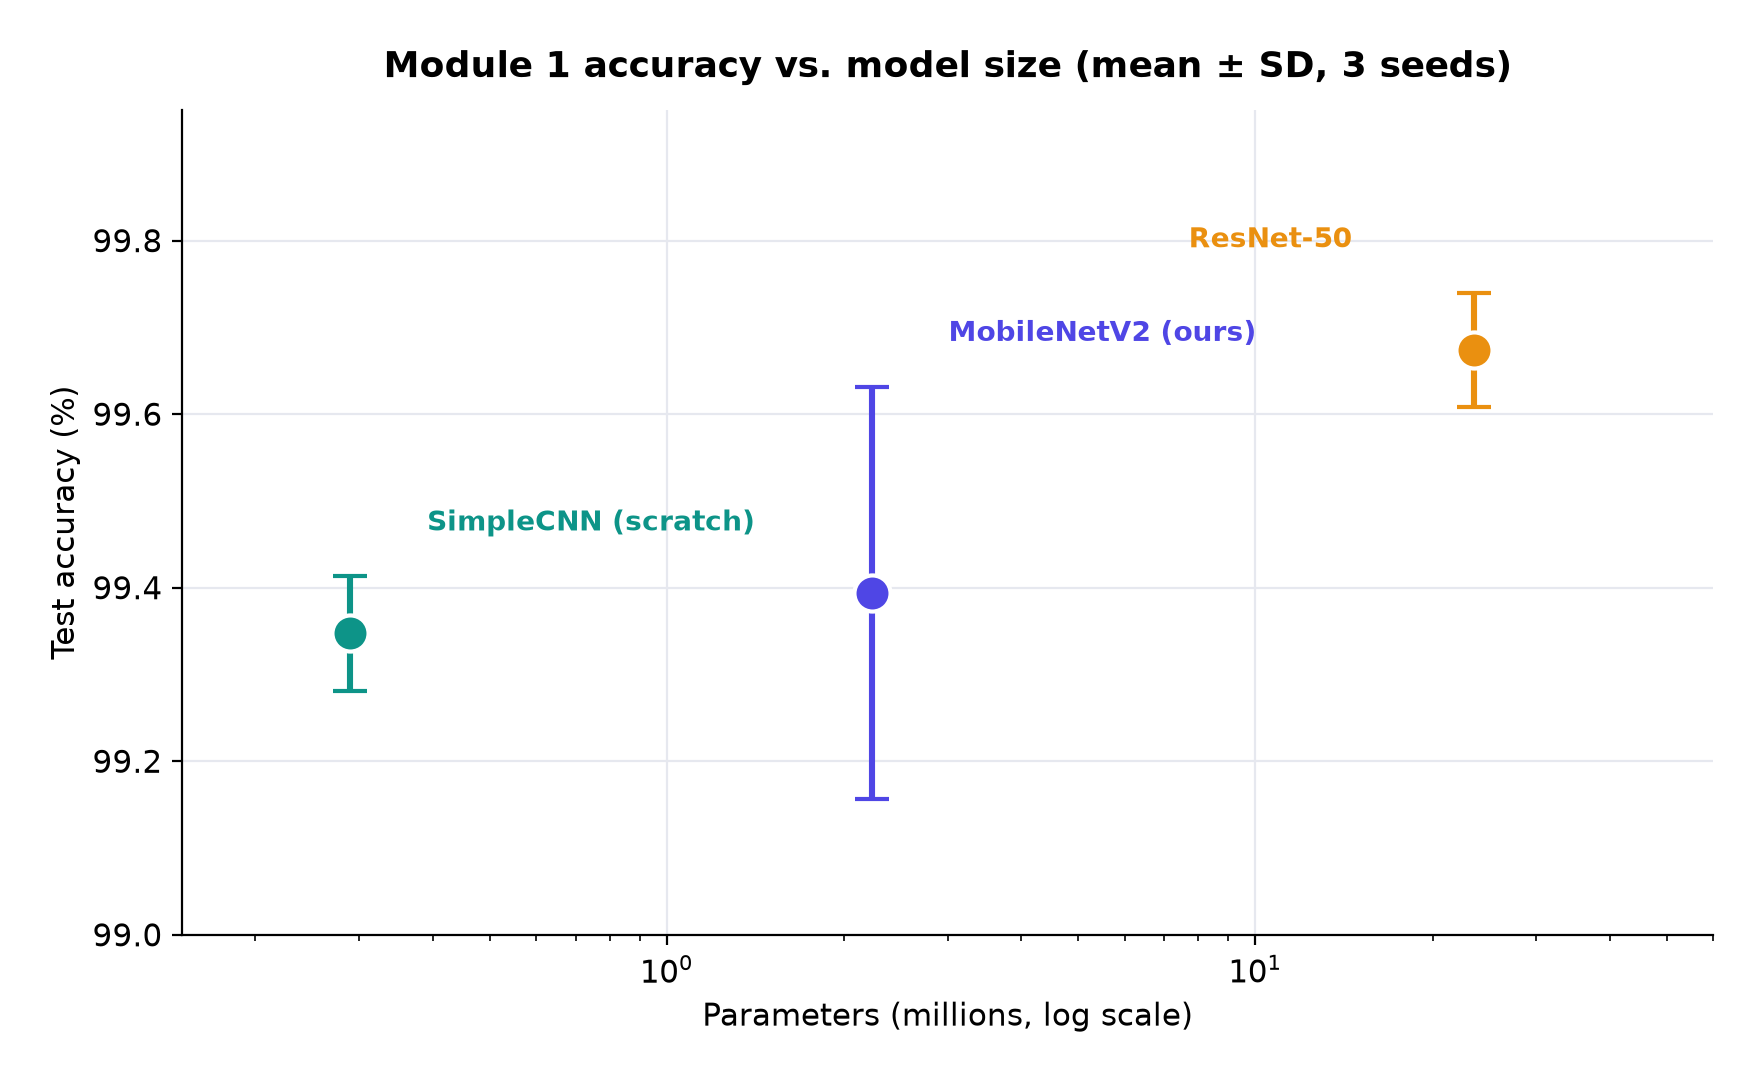
\includegraphics[width=0.78\textwidth]{fig05_m1_tradeoff.png}
\caption{Module~1 accuracy versus model size (mean $\pm$ SD over 3 seeds; note the
logarithmic parameter axis). The three error bars overlap, so the accuracy gap
between our 2.23~M-parameter MobileNetV2 and the 23.5~M-parameter ResNet-50 is not
statistically meaningful on this task---parameter efficiency, not accuracy, is what
separates the models, which is the property that matters for edge deployment.}
\label{fig:m1trade}
\end{figure}

\begin{figure}[H]
\centering
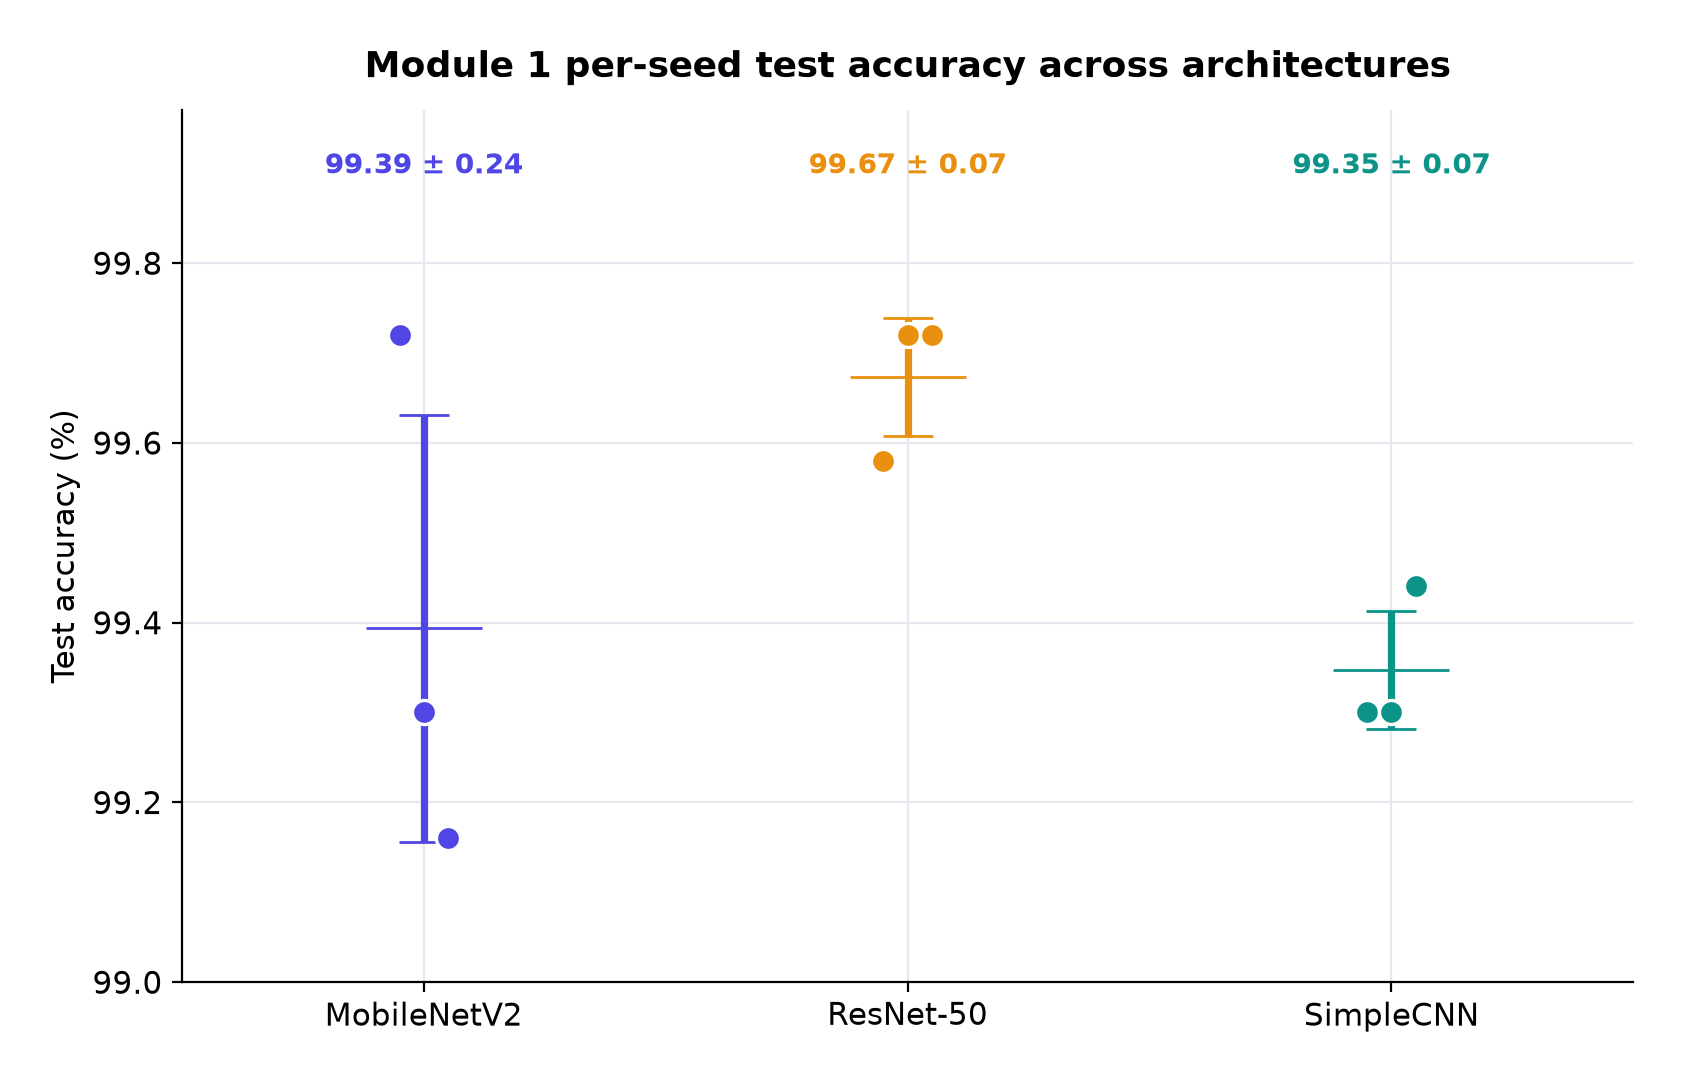
\includegraphics[width=0.78\textwidth]{fig07_m1_seed_variance.png}
\caption{Module~1 per-seed test accuracy (three seeds per architecture); each dot is
one run, the horizontal bar is the mean, and the whiskers are one standard deviation.
All three architectures cluster tightly around 99.4\%, and their spreads overlap---the
visual counterpart to the ``statistically tied'' claim, and a caution against reading
too much into any single-run number.}
\label{fig:m1seed}
\end{figure}

At the class level (Table~\ref{tab:m1class}, Figure~\ref{fig:m1cm}) precision and
recall clear 98.8\% for both classes. The number we care about is defective parts
passed as good: across seeds it ran from 2 to 5 out of 715
(Table~\ref{tab:m1seed}). Small, but not zero, and we keep it in view rather than
smooth it over. The training curves (Figures~\ref{fig:m1acc}--\ref{fig:m1loss}) show
a clean jump at the fine-tune boundary and no gap opening up between train and
validation.

\begin{table}[H]
\caption{Module~1 per-class report (median seed $s{=}2$, accuracy 99.30\%).}
\label{tab:m1class}
\centering
\small
\begin{tabular}{@{}lcccc@{}}
\toprule
Class & Precision & Recall & F1 & Support \\
\midrule
\texttt{def\_front} & 0.9956 & 0.9934 & 0.9945 & 453 \\
\texttt{ok\_front}  & 0.9886 & 0.9924 & 0.9905 & 262 \\
Macro avg    & 0.9921 & 0.9929 & 0.9925 & 715 \\
Weighted avg & 0.9930 & 0.9930 & 0.9930 & 715 \\
\bottomrule
\end{tabular}
\end{table}

\begin{table}[H]
\caption{Module~1 MobileNetV2 per-seed detail. FN = defective parts predicted
acceptable.}
\label{tab:m1seed}
\centering
\small
\begin{tabular}{@{}ccccc@{}}
\toprule
Seed & Val acc.\ (\%) & Test acc.\ (\%) & Confusion & Missed defects (FN) \\
\midrule
1  & 99.30 & 99.72 & [[451,\,2],[0,\,262]]  & 2 \\
2  & 99.30 & 99.30 & [[450,\,3],[2,\,260]]  & 3 \\
42 & 99.30 & 99.16 & [[448,\,5],[1,\,261]]  & 5 \\
\bottomrule
\end{tabular}
\end{table}

\begin{figure}[H]
\centering
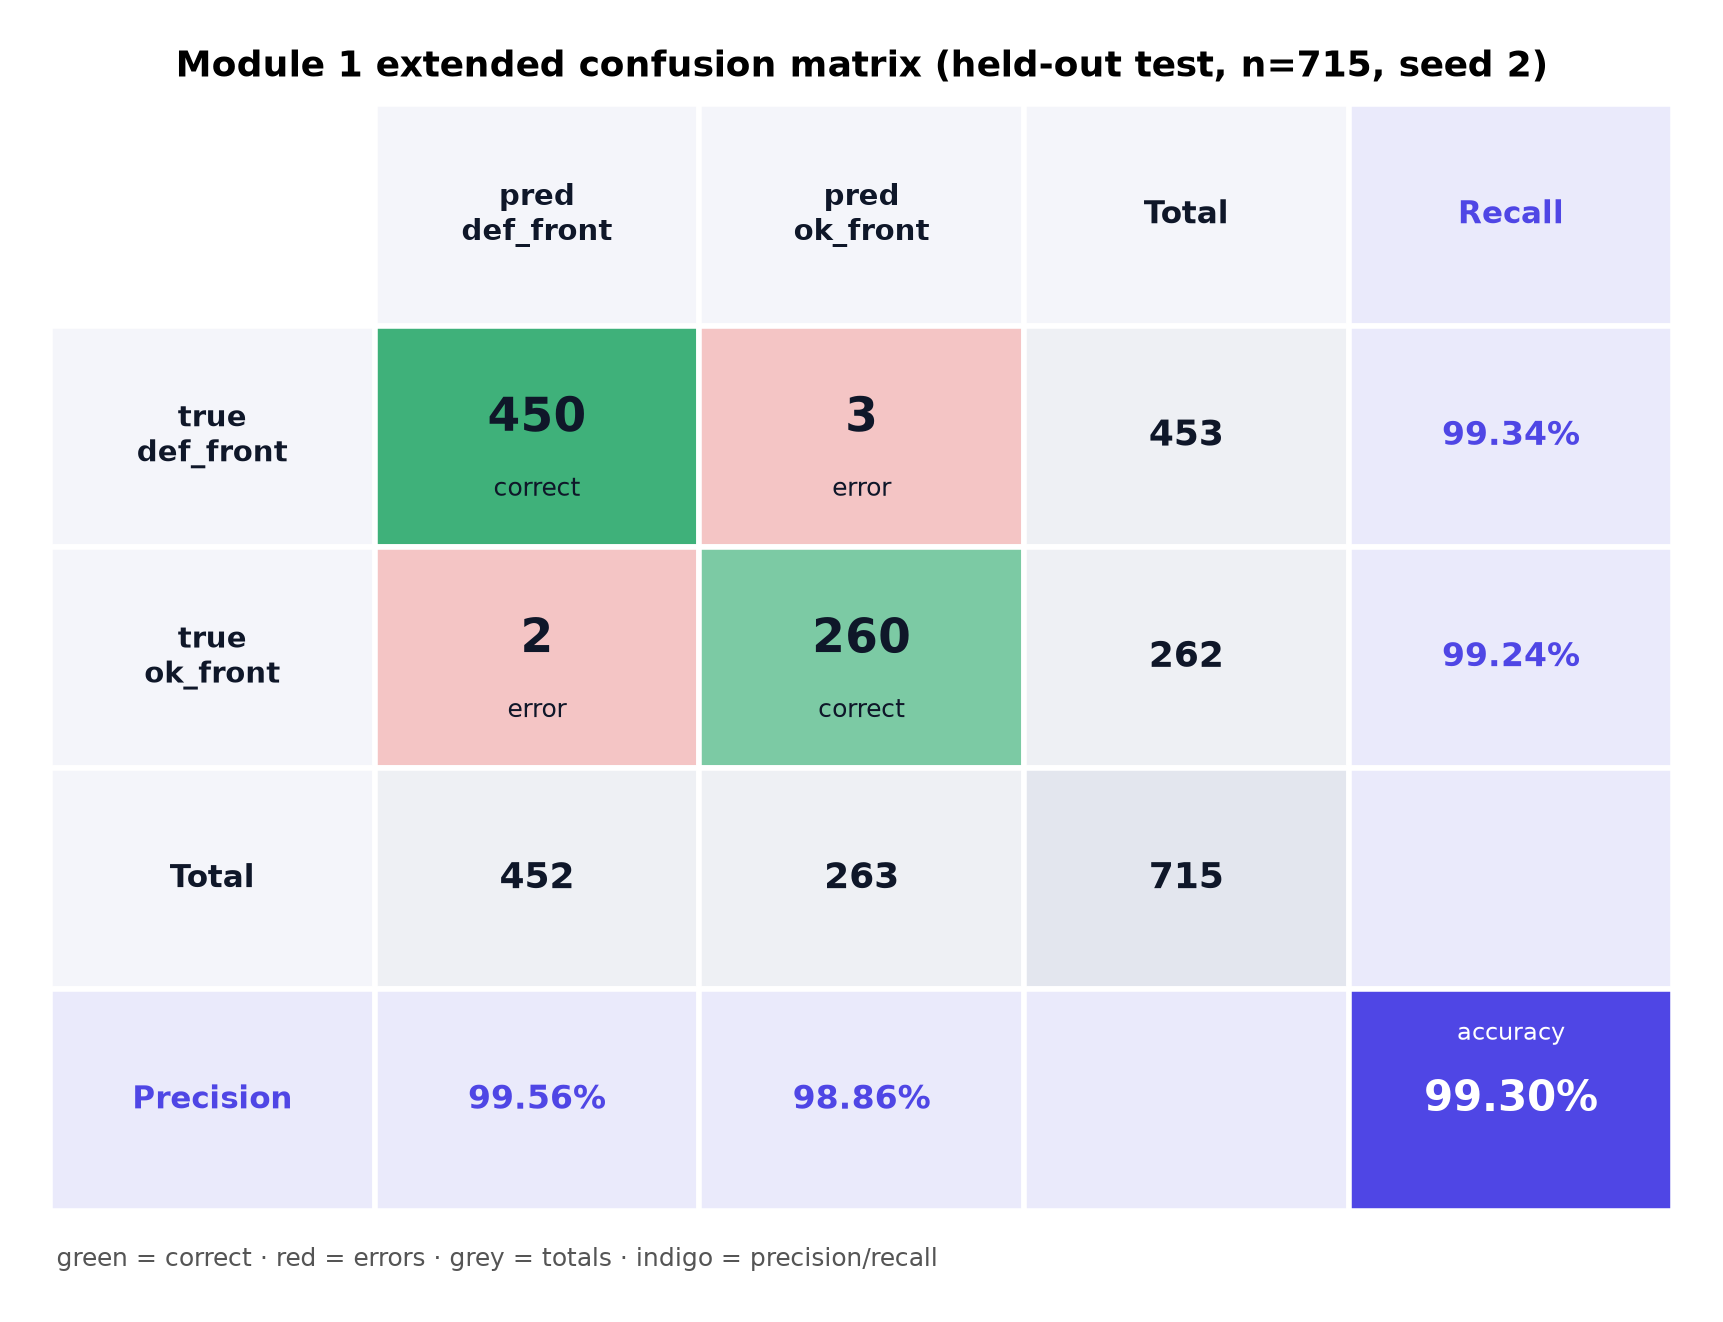
\includegraphics[width=0.72\textwidth]{fig04_m1_confusion.png}
\caption{Module~1 extended confusion matrix (held-out test, $n=715$, seed 2). Green
diagonal cells are correct predictions, red off-diagonal cells are errors, and the
grey margins give row/column totals with per-class recall and precision. Only three
defective parts were passed as acceptable (top-right) and two acceptable parts were
flagged (bottom-left); the former is the safety-critical error we track explicitly.}
\label{fig:m1cm}
\end{figure}

\begin{figure}[H]
\centering
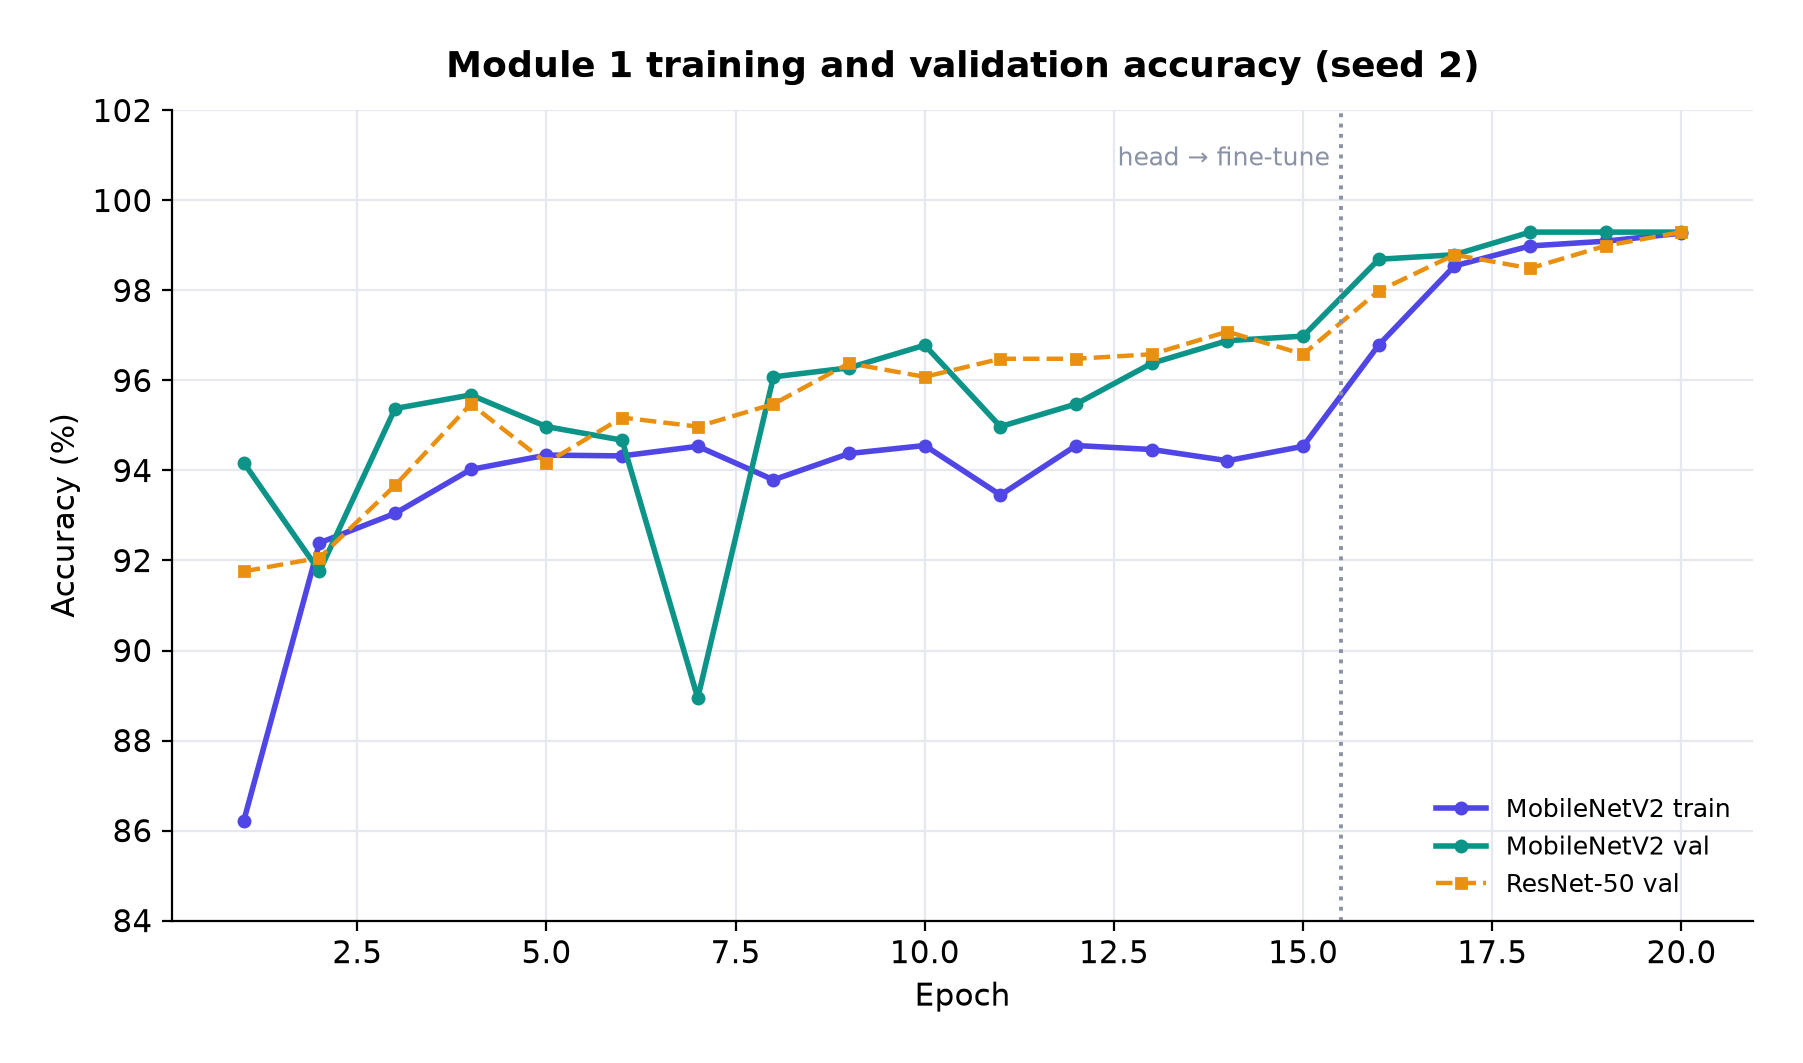
\includegraphics[width=0.85\textwidth]{fig02_m1_training_curves.png}
\caption{Module~1 training and validation accuracy over epochs (seed 2), with the
ResNet-50 validation curve for reference. The dotted line marks the switch from
frozen-backbone head training to fine-tuning, where accuracy jumps sharply as the
top layers adapt to casting images. The validation curve tracks training throughout,
indicating no overfitting despite the small dataset.}
\label{fig:m1acc}
\end{figure}

\begin{figure}[H]
\centering
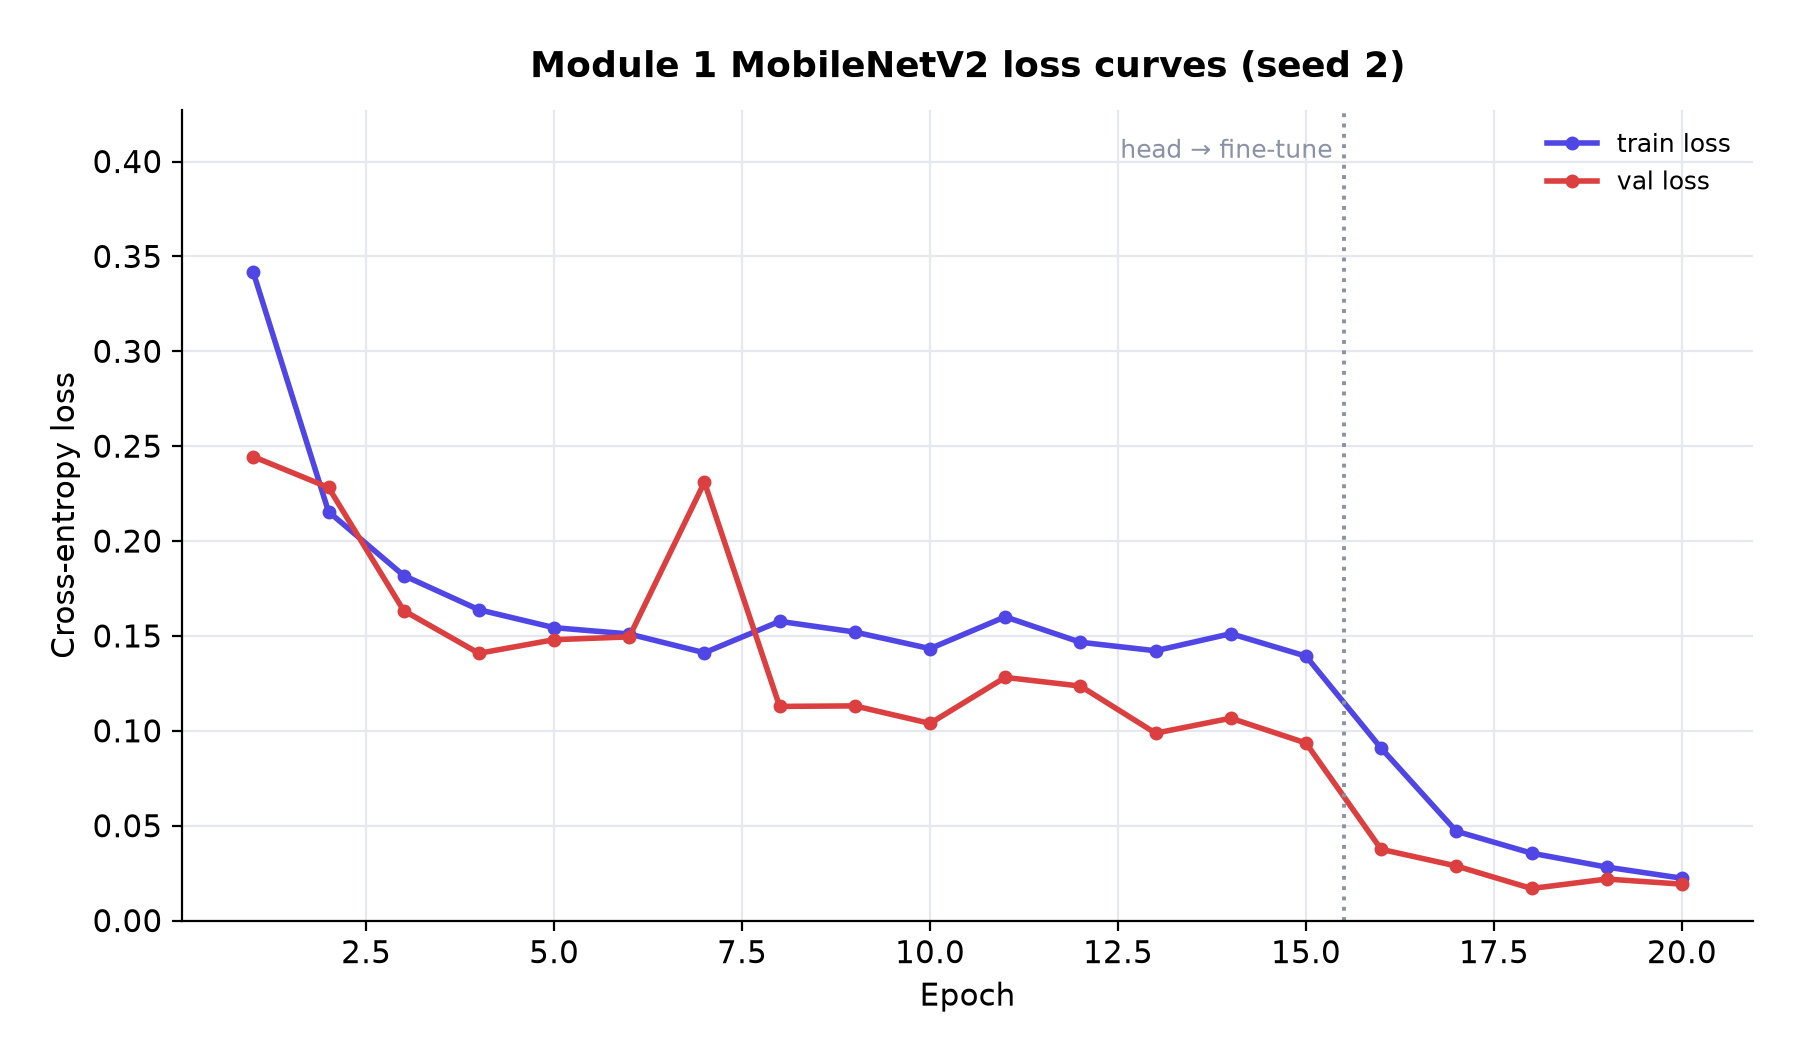
\includegraphics[width=0.85\textwidth]{fig03_m1_loss_curves.png}
\caption{Module~1 MobileNetV2 cross-entropy loss (seed 2). Training and validation
loss fall together and flatten near zero after fine-tuning begins; the absence of a
rising validation loss is further evidence the model generalizes rather than memorizes.}
\label{fig:m1loss}
\end{figure}

Latency decides whether the edge claim holds. Table~\ref{tab:m1lat} and
Figure~\ref{fig:m1lat} report single-image times (batch size 1, 30 warm-up runs, 300
timed). Through ONNX on a CPU the model averages 2.37~ms an image, with a p95 of
3.64~ms --- three orders of magnitude under the two-second budget the use case
allows, so inspection runs in real time without a GPU. Figure~\ref{fig:gradcam}
shows a Grad-CAM map: the model looks at the defect, not the background.

\begin{table}[H]
\caption{Module~1 single-image inference latency (batch=1; 30 warm-up, 300 runs).}
\label{tab:m1lat}
\centering
\small
\begin{tabular}{@{}lcc@{}}
\toprule
Configuration & Mean (ms) & p95 (ms) \\
\midrule
\textbf{ONNX Runtime, CPU (edge target)} & \textbf{2.37} & 3.64 \\
PyTorch, GPU & 8.07 & 12.98 \\
PyTorch, CPU & 12.39 & 13.99 \\
\bottomrule
\end{tabular}
\end{table}

\begin{figure}[H]
\centering
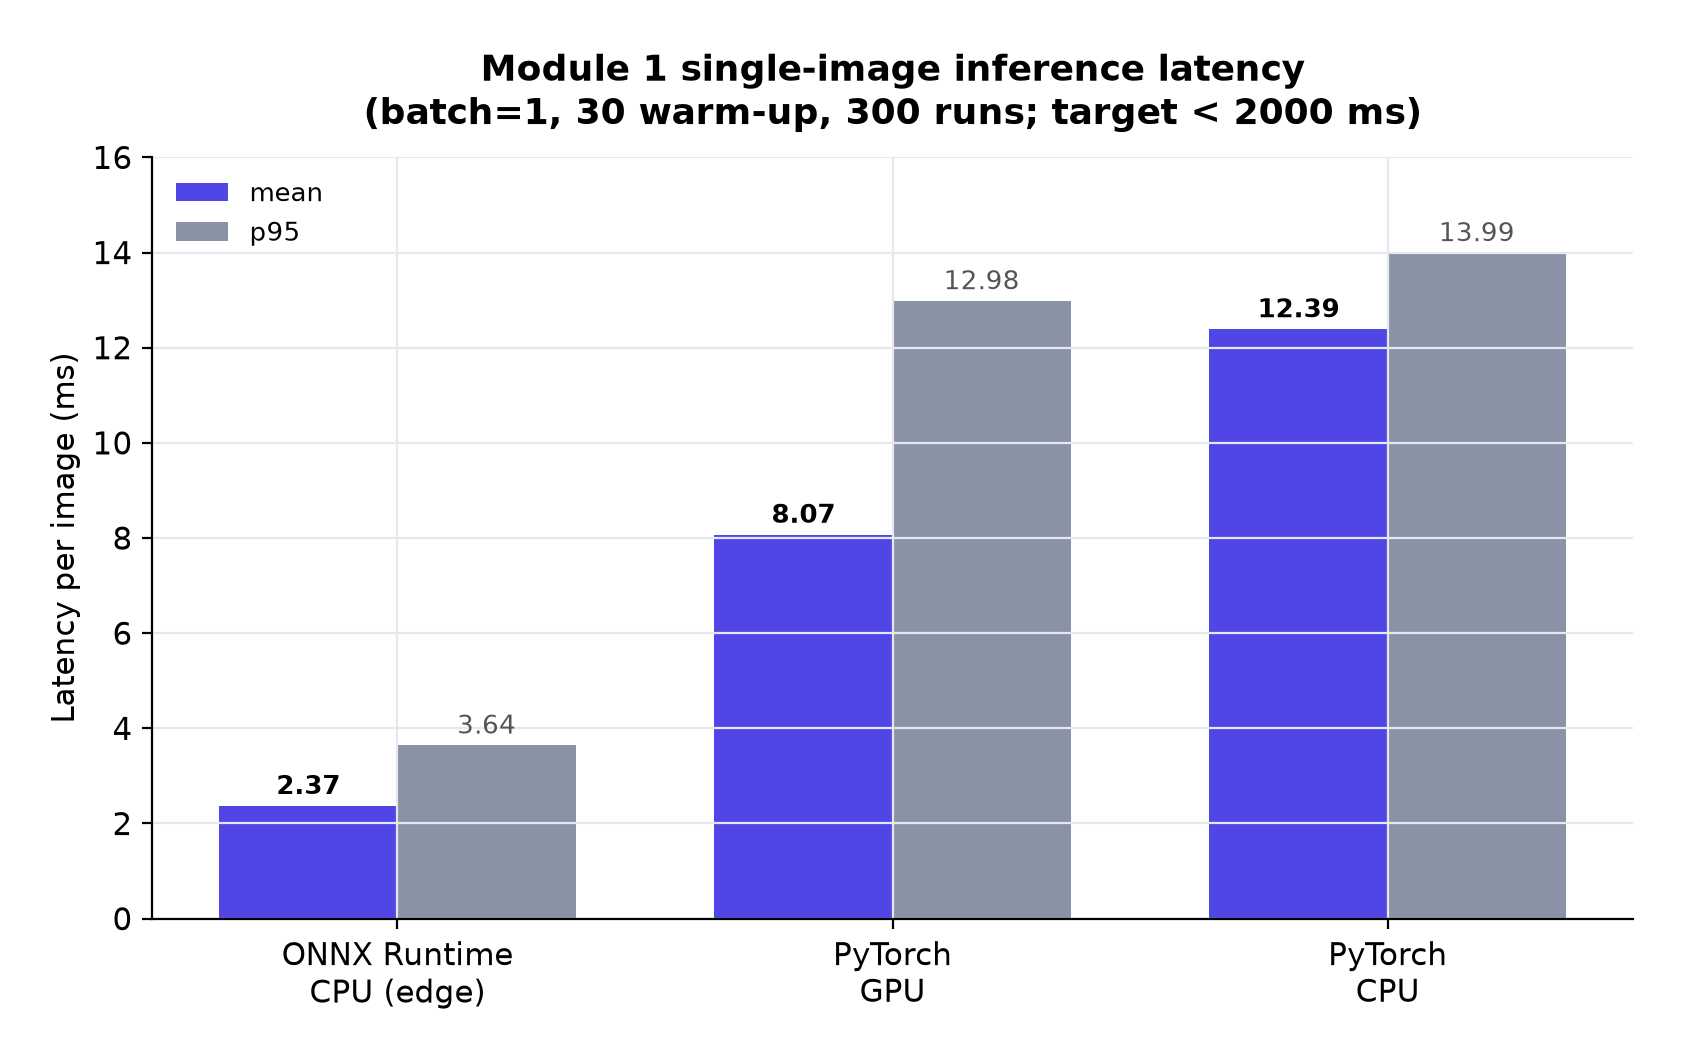
\includegraphics[width=0.75\textwidth]{fig06_m1_latency.png}
\caption{Module~1 single-image inference latency across runtimes (mean and p95 bars).
Exporting to ONNX and running on CPU is about five times faster than the native PyTorch
CPU path and even beats the GPU at batch size~1, because it avoids framework and
data-transfer overhead. This is what makes GPU-free, real-time inspection practical on
an MSME shop floor.}
\label{fig:m1lat}
\end{figure}

\begin{figure}[H]
\centering
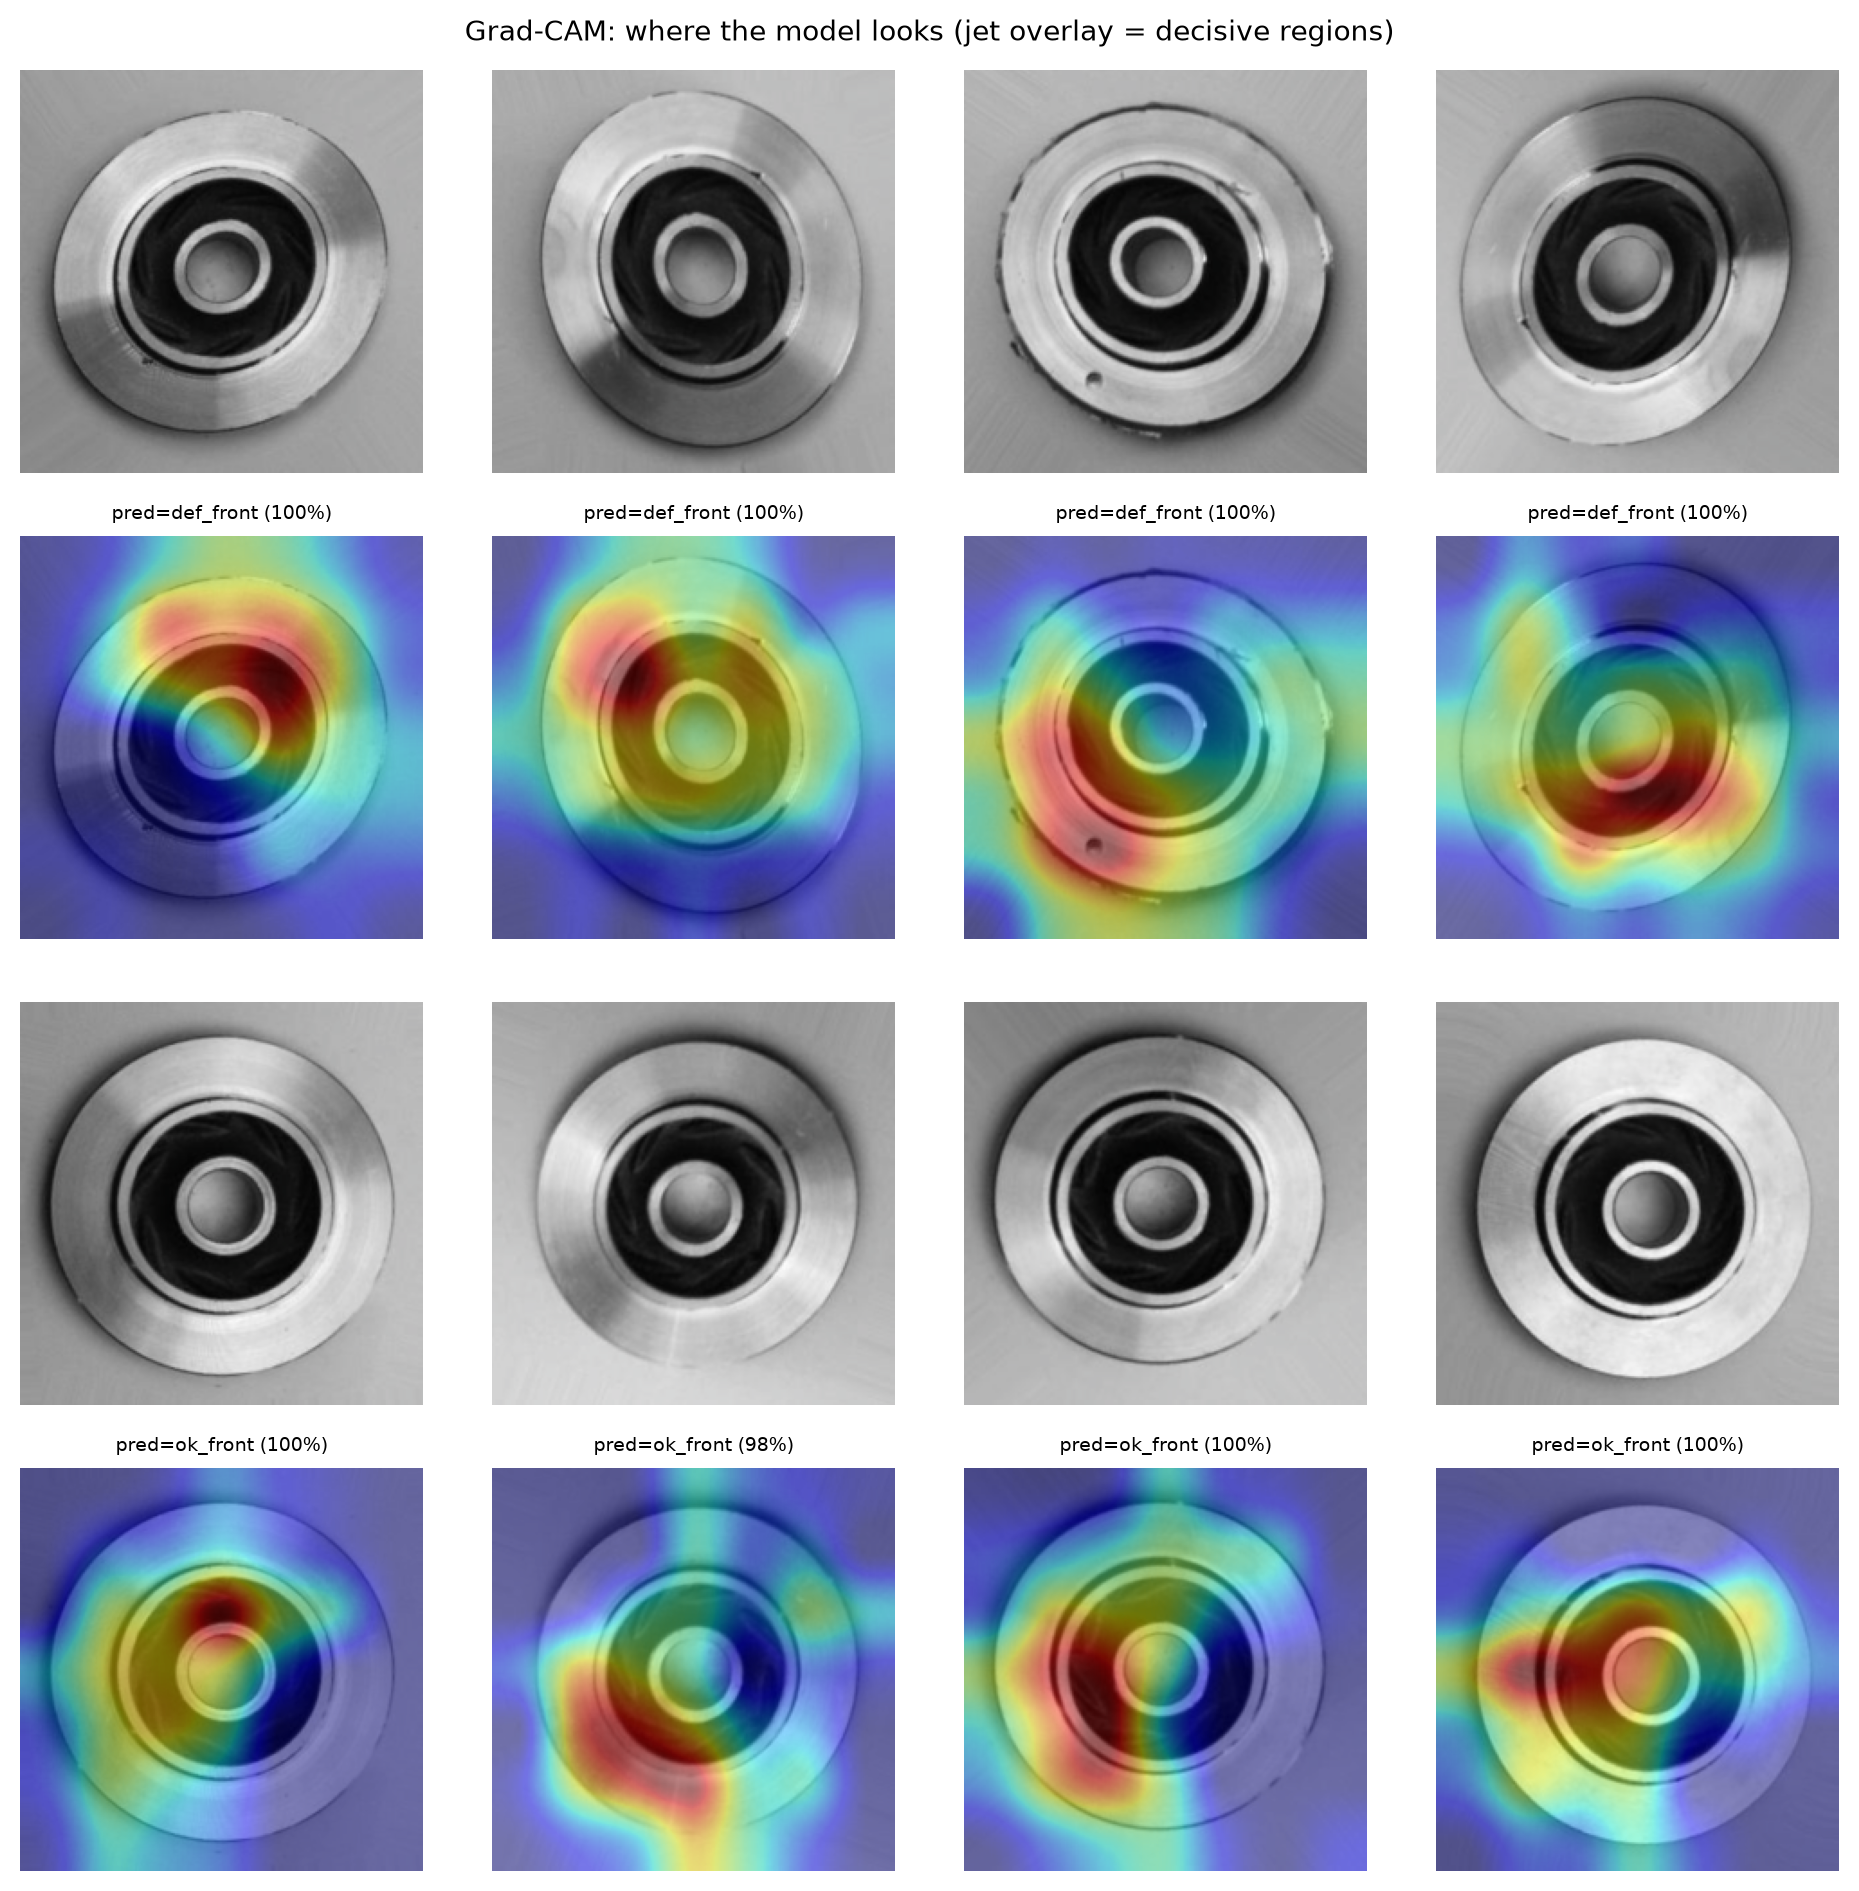
\includegraphics[width=0.62\textwidth]{gradcam.png}
\caption{Module~1 Grad-CAM saliency: each pair shows an input casting (top) and the
class-activation heat map (bottom), where warmer colours mark the pixels most
responsible for the prediction. The model concentrates on the actual surface anomaly
rather than the background or part edges, evidence that it learned the defect itself
and not a dataset shortcut---important for trust on the shop floor.}
\label{fig:gradcam}
\end{figure}

\subsection{Module 3 --- Predictive maintenance}
\label{sec:res-m3}

On the by-tool split the XGBoost regressor gets RMSE 0.199, MAE 0.160, and
$R^2 = 0.545$ on the four unseen tools --- about double the linear model's $R^2$ and
well past the constant-mean floor (Table~\ref{tab:m3res}, Figure~\ref{fig:m3cmp}). A
middling $R^2$ is the honest number here. Guessing the wear path of a tool the model
has never met is hard, and a much higher score under a random split would point to
leakage rather than skill. Figure~\ref{fig:m3pa} plots prediction against truth for
each test tool: the model follows the wear trend, with the per-tool scatter you
would expect.

\begin{table}[H]
\caption{Module~3 RUL regression versus baselines on unseen test tools. The constant-mean
row is the no-skill reference ($R^2\approx0$); XGBoost roughly doubles the linear model's
$R^2$ and cuts its error, confirming it learns non-linear wear structure rather than a
simple trend.}
\label{tab:m3res}
\centering
\small
\begin{tabular}{@{}lccc@{}}
\toprule
Model & RMSE $\downarrow$ & MAE $\downarrow$ & $R^2$ $\uparrow$ \\
\midrule
Constant mean (no-skill) & 0.2955 & 0.2562 & $-0.000$ \\
Linear regression & 0.2534 & 0.1941 & 0.2647 \\
\textbf{XGBoost (ours)} & \textbf{0.1995} & \textbf{0.1602} & \textbf{0.5445} \\
\bottomrule
\end{tabular}
\end{table}

\begin{figure}[H]
\centering
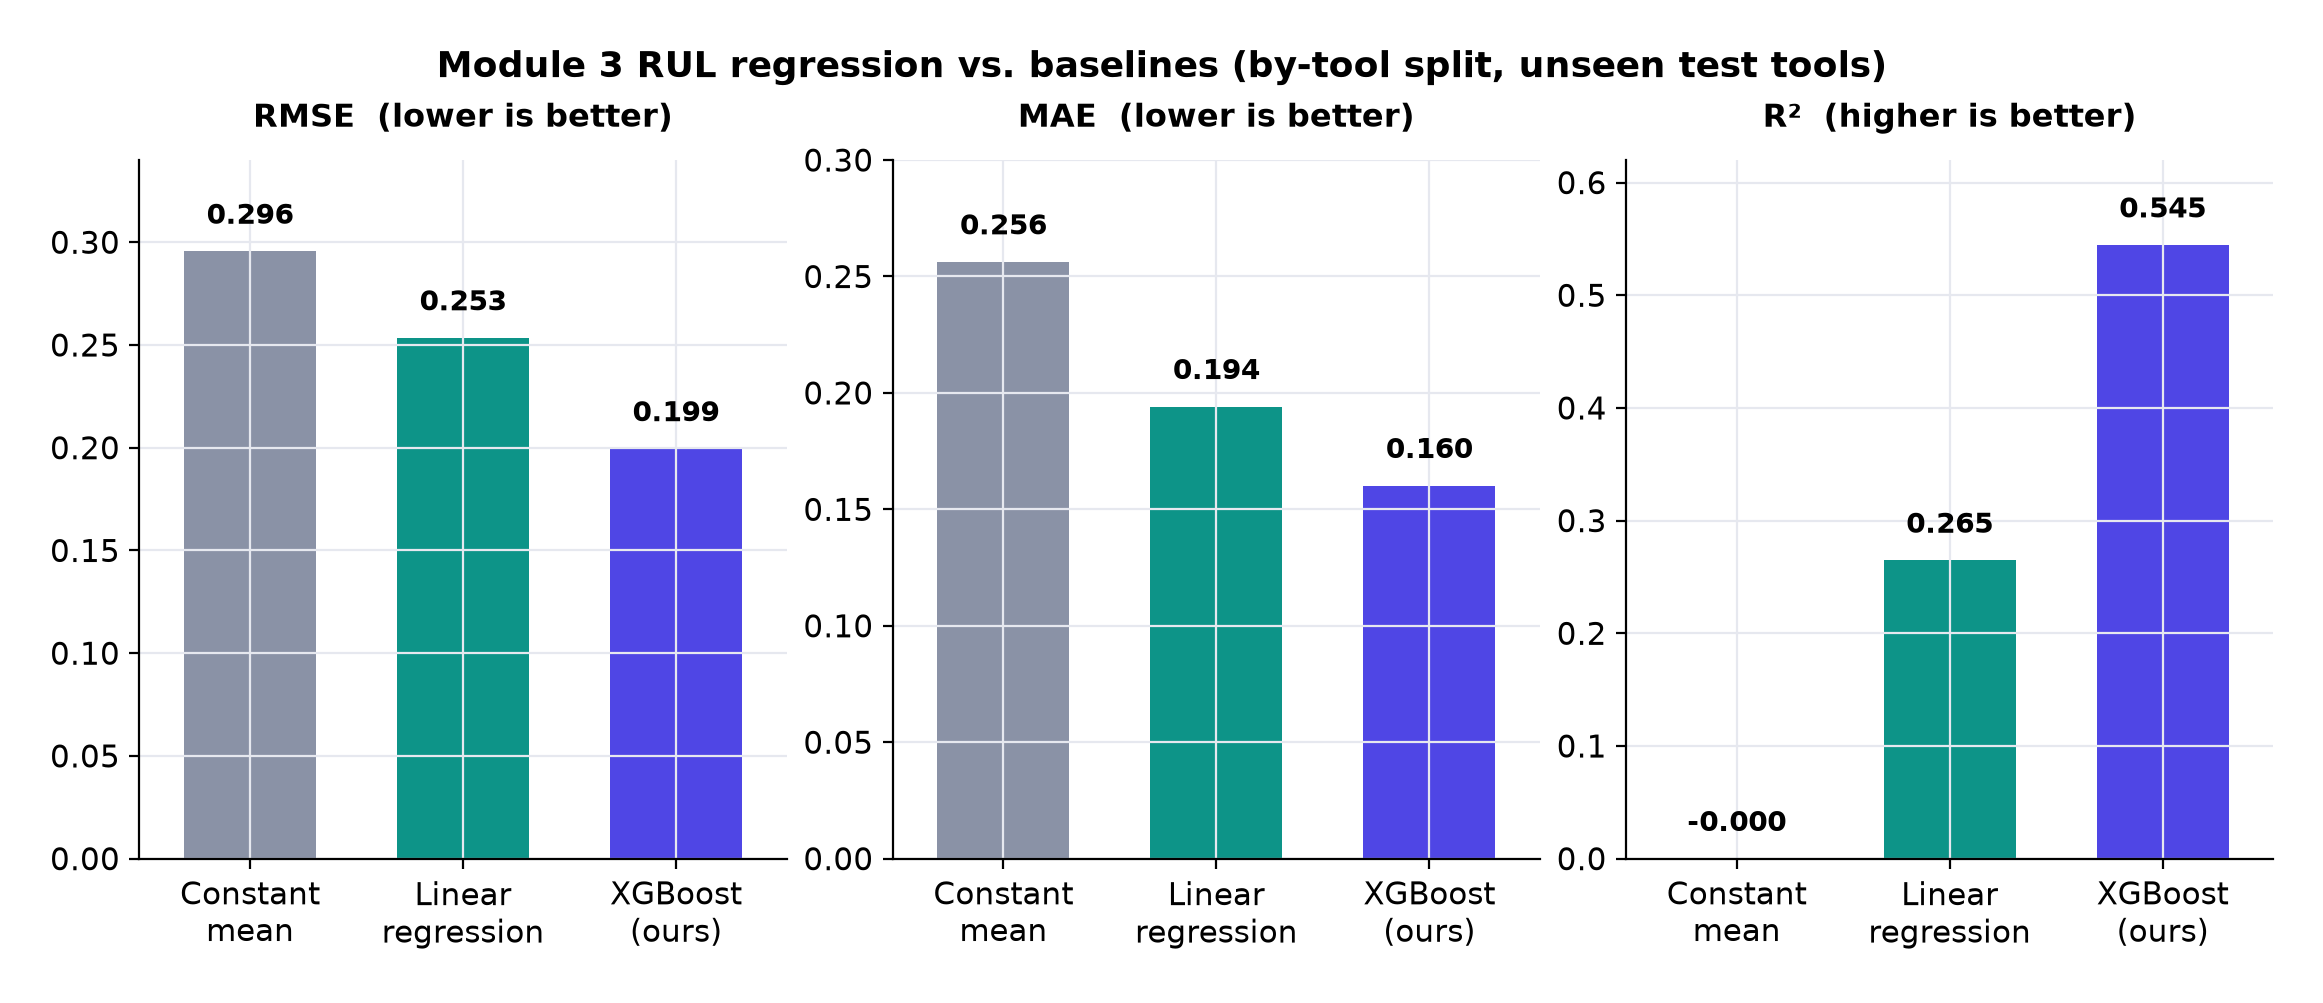
\includegraphics[width=\textwidth]{fig08_m3_comparison.png}
\caption{Module~3 RUL regression versus baselines on the by-tool split, across three
metrics (lower is better for RMSE and MAE; higher is better for $R^2$). XGBoost improves
on both the no-skill constant-mean predictor and the linear model on every metric,
and roughly doubles the linear model's $R^2$---the clearest sign it captures non-linear
wear structure that a linear fit cannot.}
\label{fig:m3cmp}
\end{figure}

\begin{figure}[H]
\centering
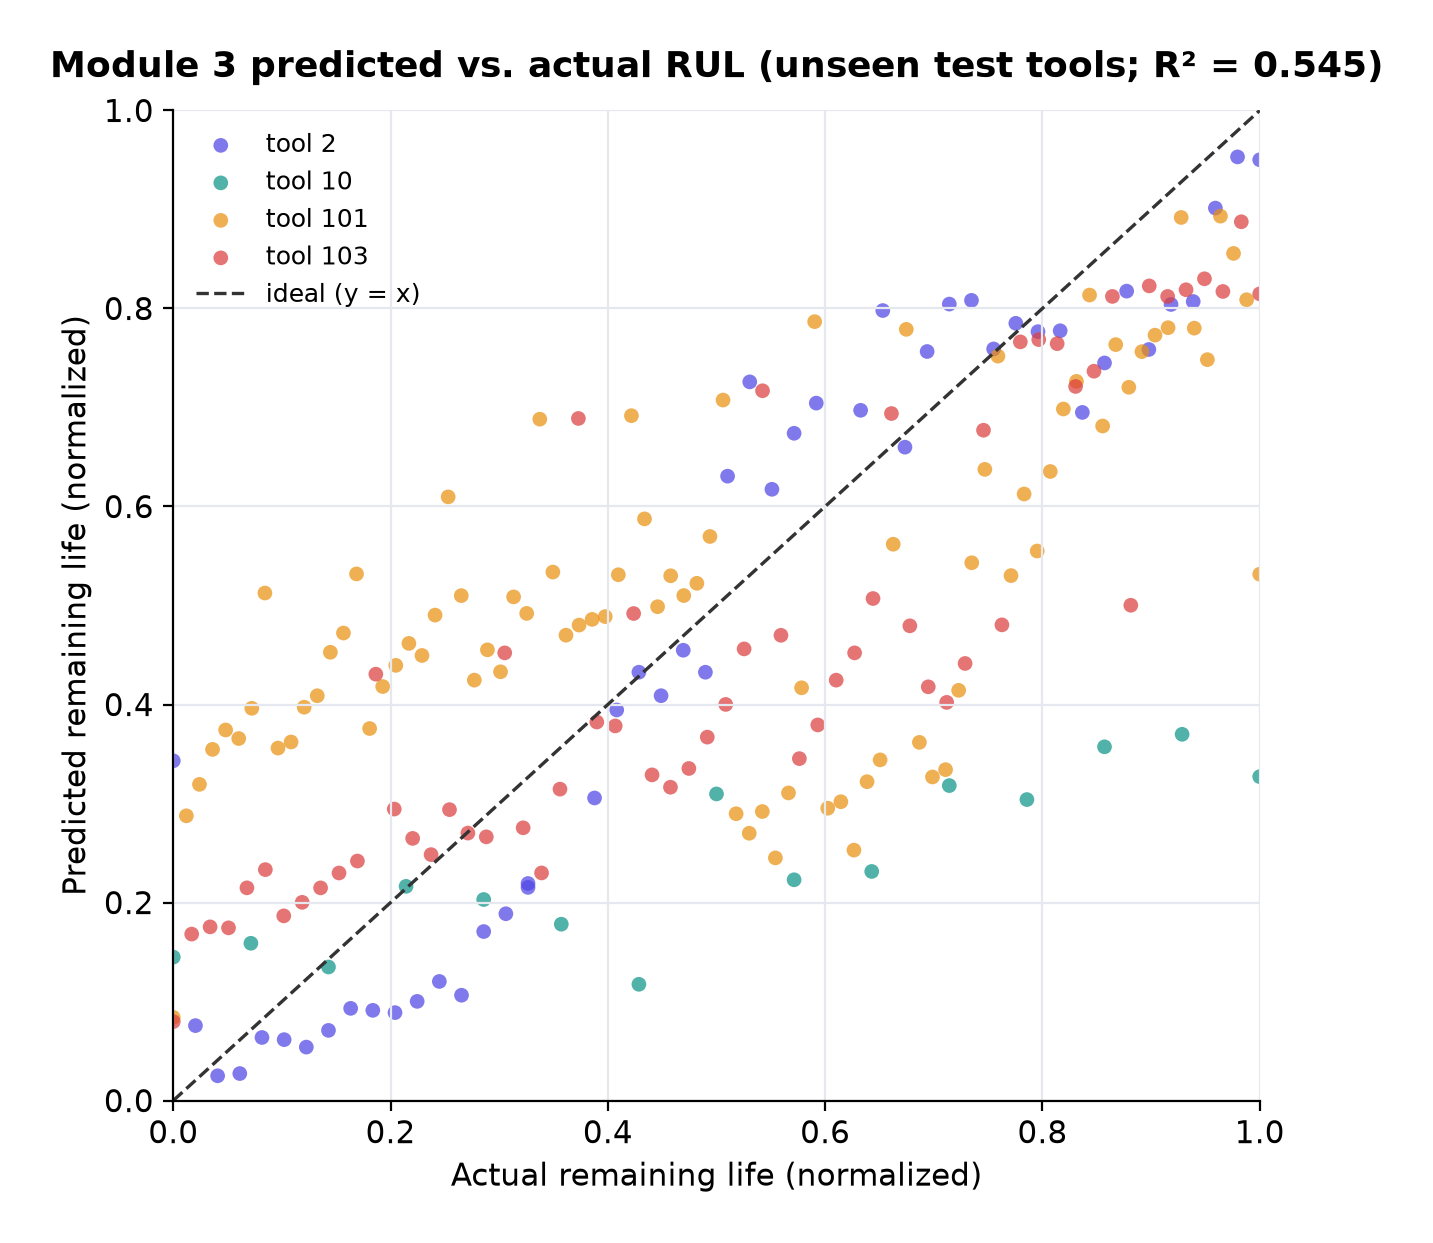
\includegraphics[width=0.62\textwidth]{fig09_m3_pred_actual.png}
\caption{Module~3 predicted versus actual normalized remaining life on the four unseen
test tools ($R^2 = 0.545$), coloured by tool; points on the dashed $y=x$ line are perfect
predictions. The cloud follows the diagonal---the model captures the overall wear
trend---but with visible per-tool scatter, the honest signature of generalizing to tools
whose exact wear signature was never seen in training.}
\label{fig:m3pa}
\end{figure}

\subsection{Module 4 --- Demand forecasting}
\label{sec:res-m4}

Over the 52 held-out weeks the XGBoost forecaster reaches 19.7\% WAPE --- 23\%
better than the naïve last-value baseline and well clear of seasonal-naïve (27.8\%)
and Prophet (30.4\%) (Table~\ref{tab:m4res}, Figure~\ref{fig:m4wape}). Beating every
baseline, Prophet included, says the model has picked up real timing in the data
instead of parroting the last week. The rest of the numbers back this up
(Table~\ref{tab:m4supp}): an $R^2$ of 0.944 and a three-fold expanding-window WAPE of
20.6\% (Table~\ref{tab:m4cv}, Figure~\ref{fig:m4cv}), close to the final held-out
figure, so the result holds across time rather than riding one lucky split.

\begin{table}[H]
\caption{Module~4 forecaster versus baselines (held-out 52 weeks, 28 categories). The
final column is the relative change in WAPE against the naïve last-value baseline:
seasonal-naïve and Prophet are actually \emph{worse} than naïve on this data, while our
XGBoost model improves on it by 23\%.}
\label{tab:m4res}
\centering
\small
\begin{tabular}{@{}lcc@{}}
\toprule
Forecaster & WAPE (\%) $\downarrow$ & Rel.\ vs.\ naïve \\
\midrule
Prophet & 30.39 & $-18.4\%$ \\
Seasonal-naïve (52-week) & 27.77 & $-8.2\%$ \\
Naïve (last value) & 25.66 & --- \\
\textbf{XGBoost (ours)} & \textbf{19.74} & \textbf{$+23.1\%$} \\
\bottomrule
\end{tabular}
\end{table}

\begin{table}[H]
\caption{Module~4 supporting metrics (final held-out model).}
\label{tab:m4supp}
\centering
\small
\begin{tabular}{@{}lcc@{}}
\toprule
Metric & Value & Note \\
\midrule
WAPE & 19.74\% & future weeks \\
$R^2$ & 0.9438 & held-out weeks \\
RMSE / MAE & 722{,}263 / 142{,}354 & units \\
Cross-val WAPE (3-fold) & 20.60\% & expanding window \\
Interval coverage & 74.20\% & target $\approx 80\%$ \\
\bottomrule
\end{tabular}
\end{table}

\begin{table}[H]
\caption{Module~4 expanding-window cross-validation.}
\label{tab:m4cv}
\centering
\small
\begin{tabular}{@{}lc@{}}
\toprule
Fold & WAPE (\%) \\
\midrule
Fold 1 & 22.7 \\
Fold 2 & 17.4 \\
Fold 3 & 21.7 \\
\textbf{Mean} & \textbf{20.6} \\
Final held-out & 19.7 \\
\bottomrule
\end{tabular}
\end{table}

\begin{figure}[H]
\centering
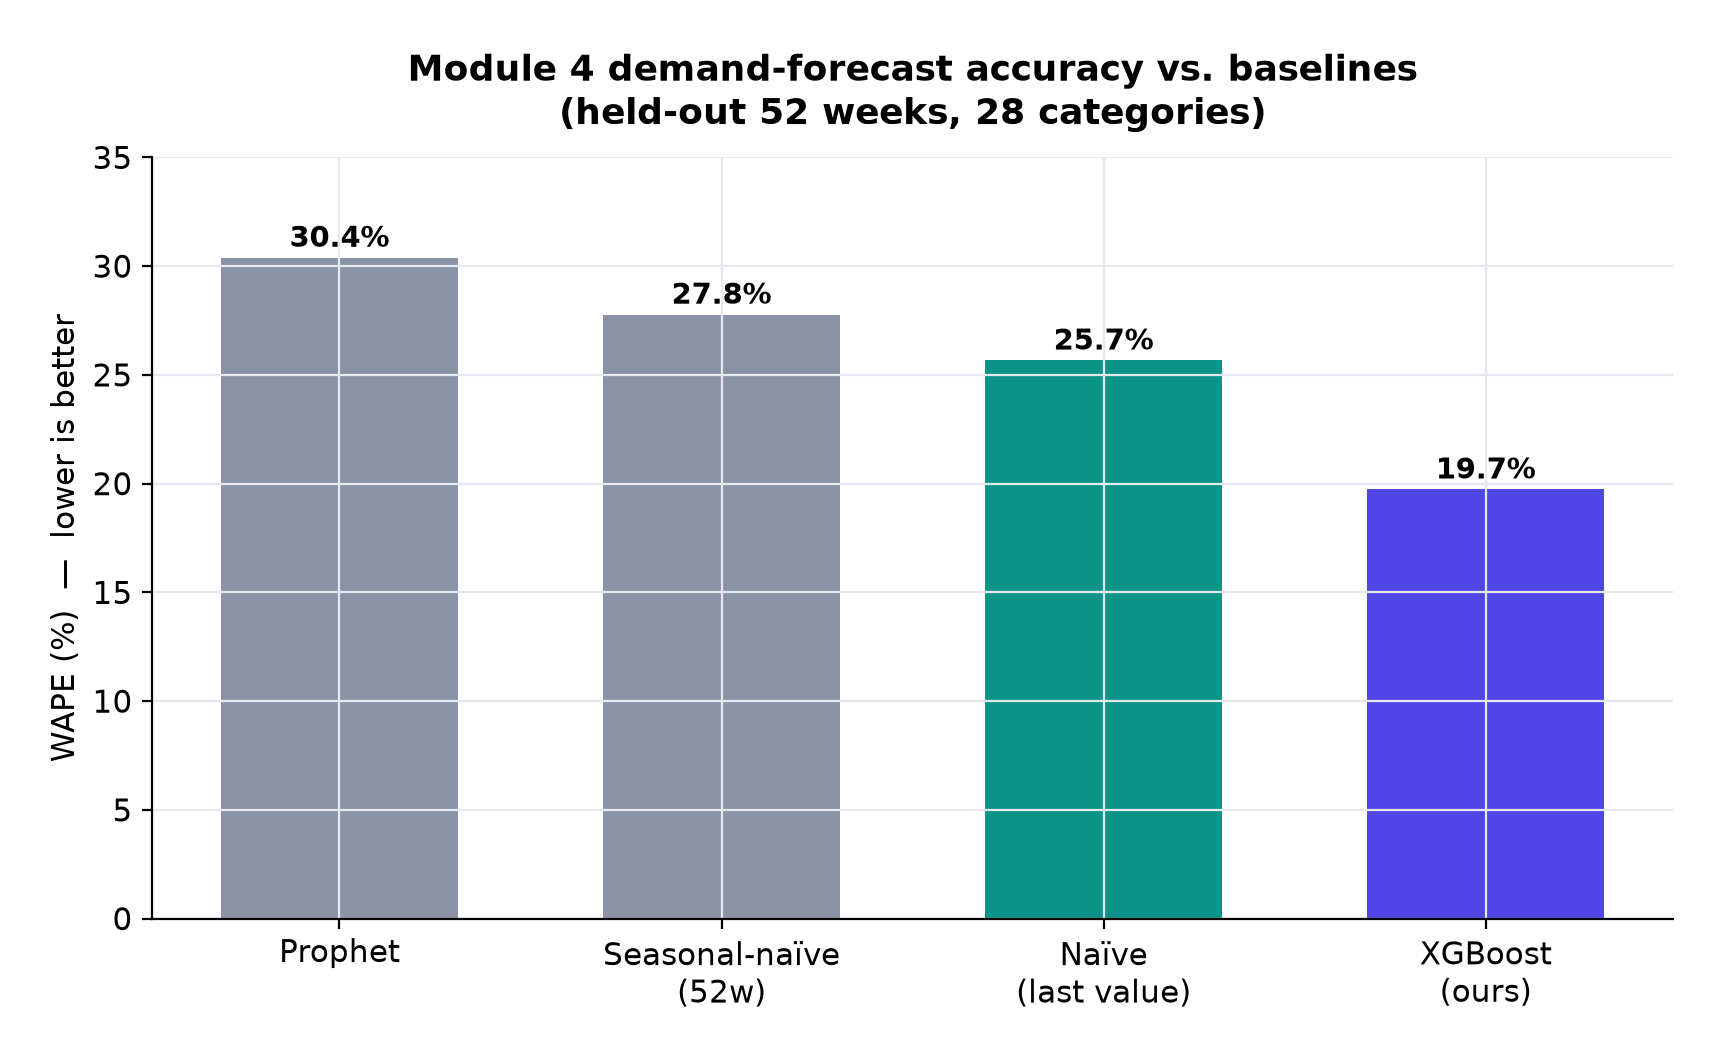
\includegraphics[width=0.82\textwidth]{fig10_m4_wape.png}
\caption{Module~4 demand-forecast accuracy versus baselines (lower WAPE is better).
The XGBoost model is well below not only the naïve and seasonal-naïve baselines but
also Prophet, a strong automatic forecaster---so the gain reflects genuinely learned
temporal structure, not merely echoing the most recent week.}
\label{fig:m4wape}
\end{figure}

\begin{figure}[H]
\centering
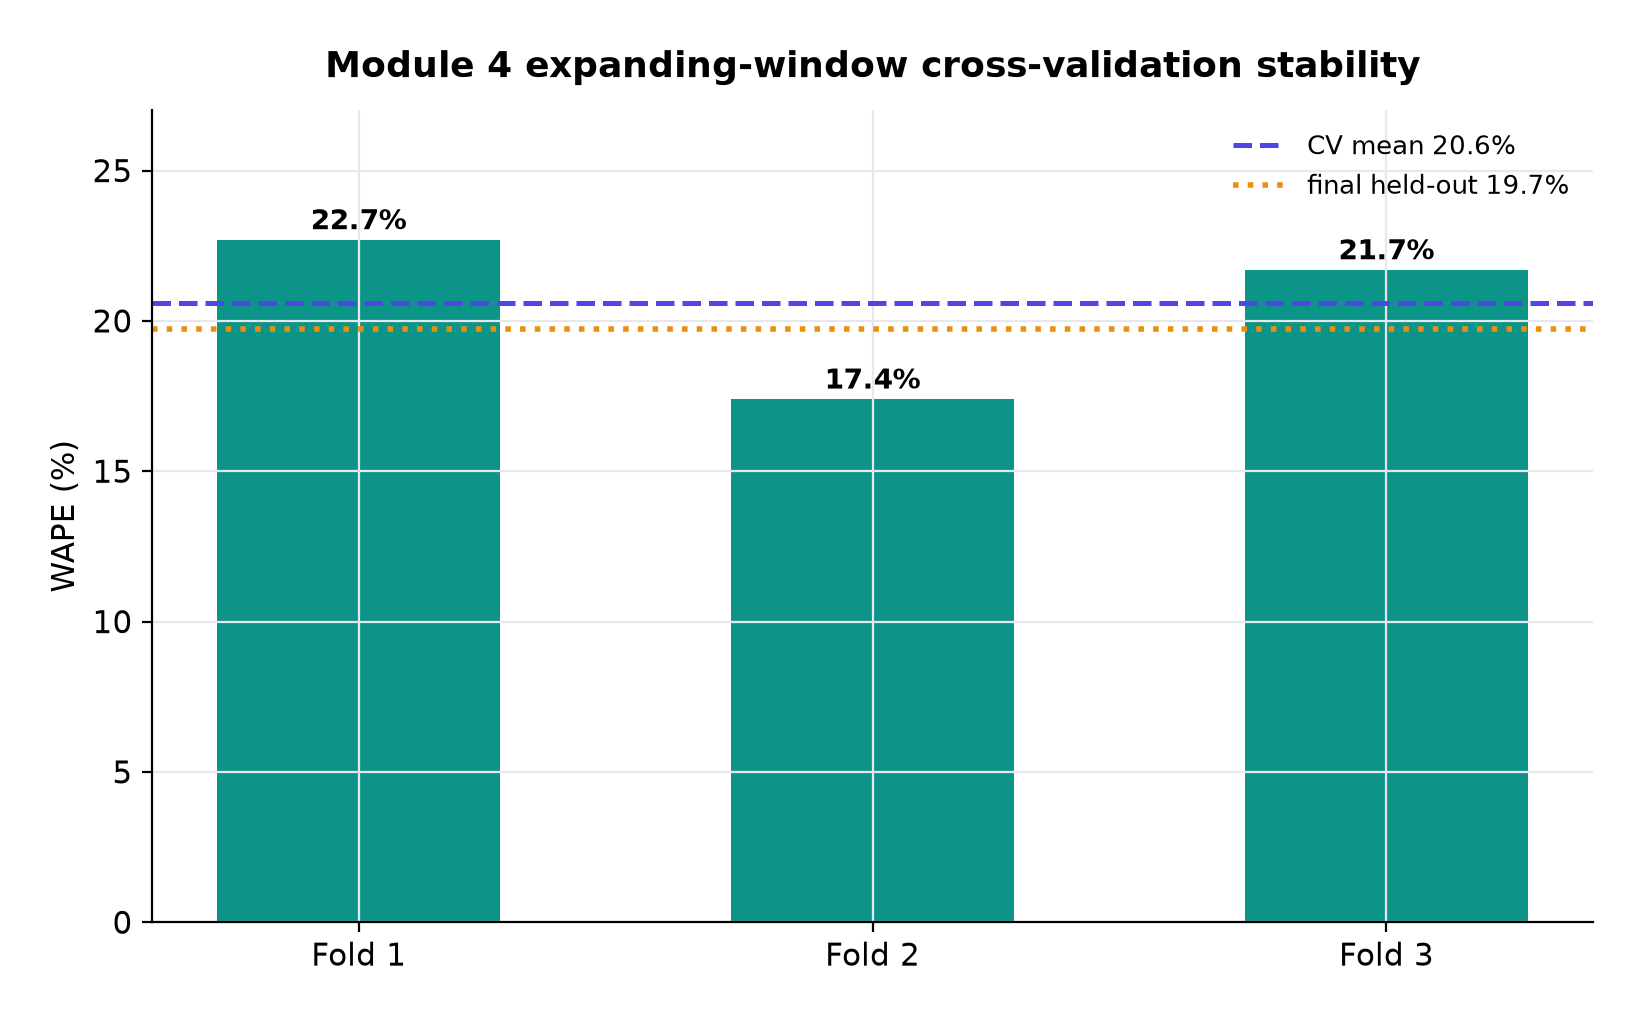
\includegraphics[width=0.78\textwidth]{fig11_m4_cv.png}
\caption{Module~4 expanding-window cross-validation WAPE across three time folds. The
dashed line is the cross-validation mean (20.6\%) and the dotted line the final
held-out score (19.7\%). The folds stay in a narrow 17--23\% band and bracket the final
number, showing the result is stable over time and not a lucky single split.}
\label{fig:m4cv}
\end{figure}

The paired quantile models give an 80\% band that actually covers 74.2\% of the
time --- a little tight of the 80\% target, and we report it that way.
Figure~\ref{fig:m4fc} shows one category's forecast with its band, and
Figure~\ref{fig:m4imp} shows short-window rolling means at the top of the feature
importance, which fits the idea that demand is easiest to read off its own recent,
smoothed level.

\begin{figure}[H]
\centering
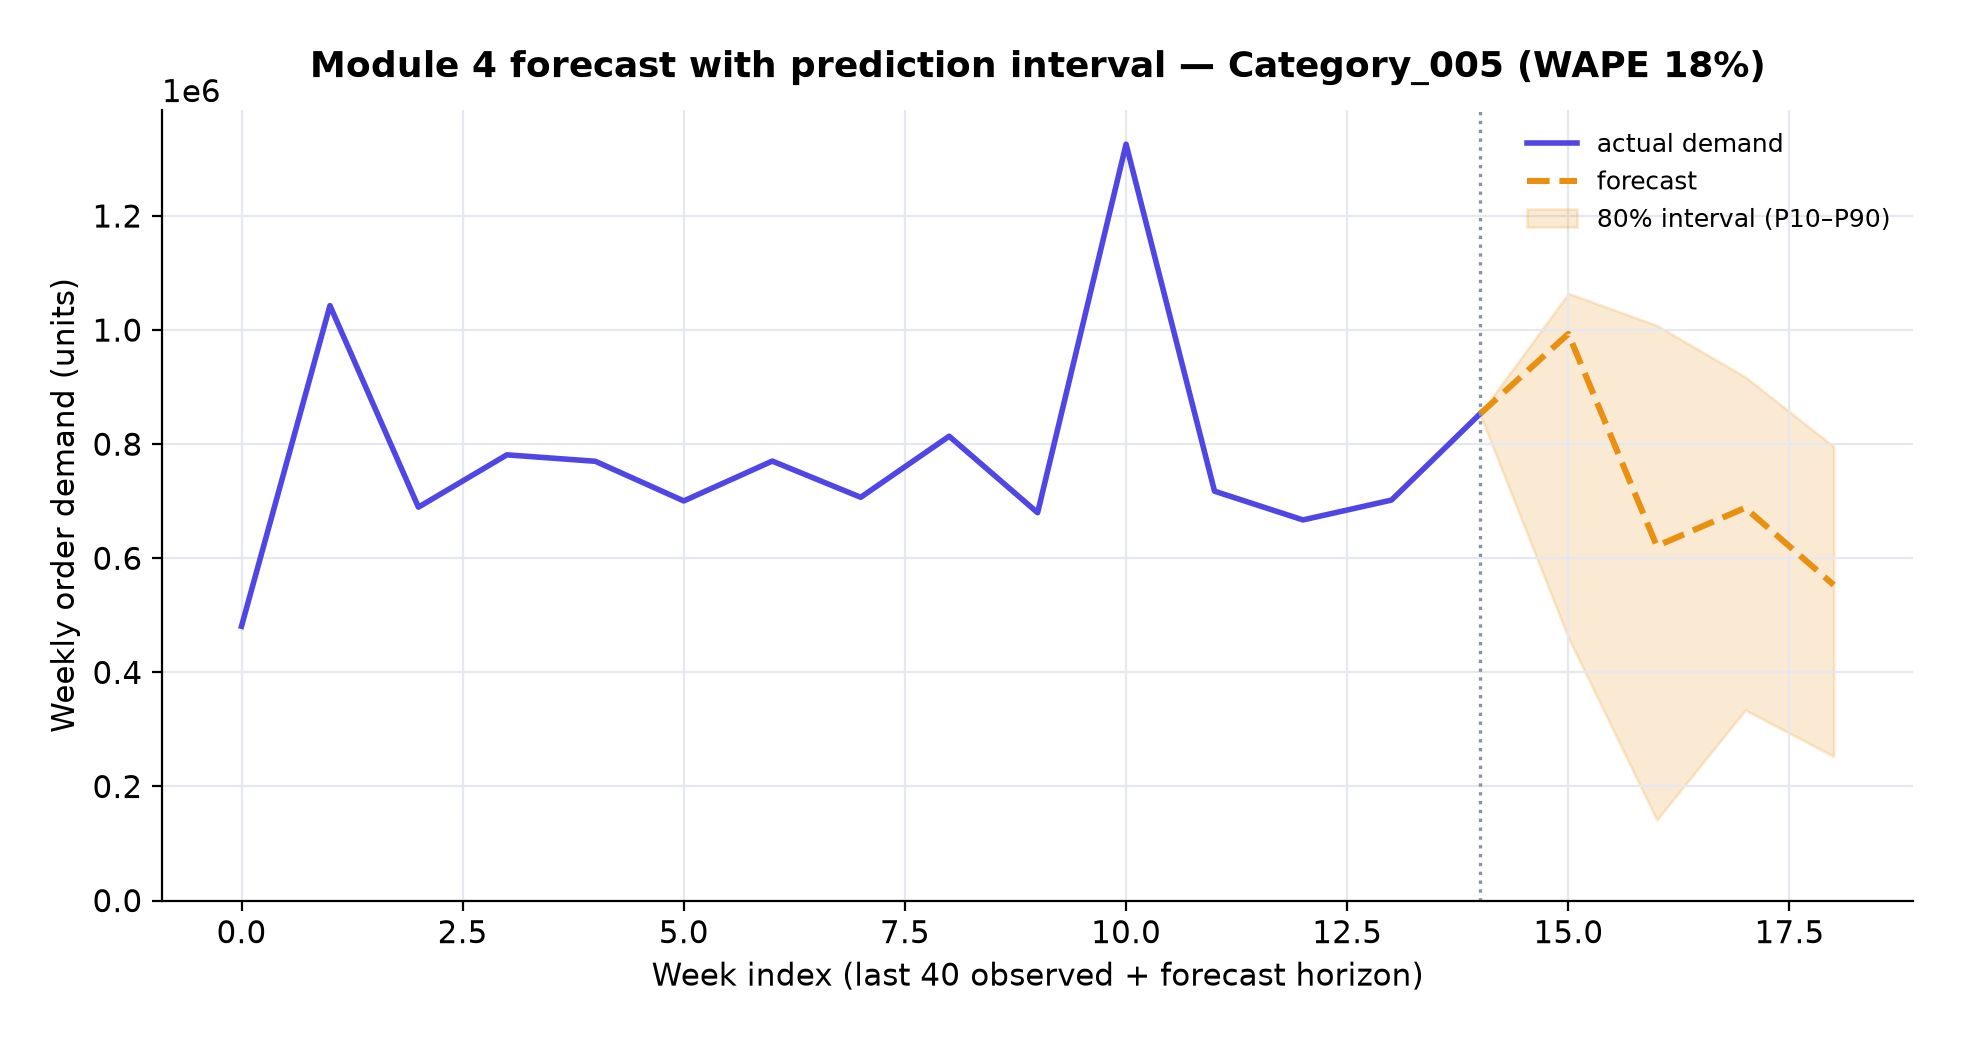
\includegraphics[width=0.85\textwidth]{fig12_m4_forecast.png}
\caption{Module~4 forecast with an 80\% P10--P90 prediction interval for a
representative category. The solid line is observed weekly demand, the dashed line the
forecast, and the shaded band the P10--P90 interval; the band widens with the forecast
horizon, correctly expressing growing uncertainty further into the future. (Truncated
final observed weeks, an artifact of the source data, are trimmed here---see caveat L6.)}
\label{fig:m4fc}
\end{figure}

\begin{figure}[H]
\centering
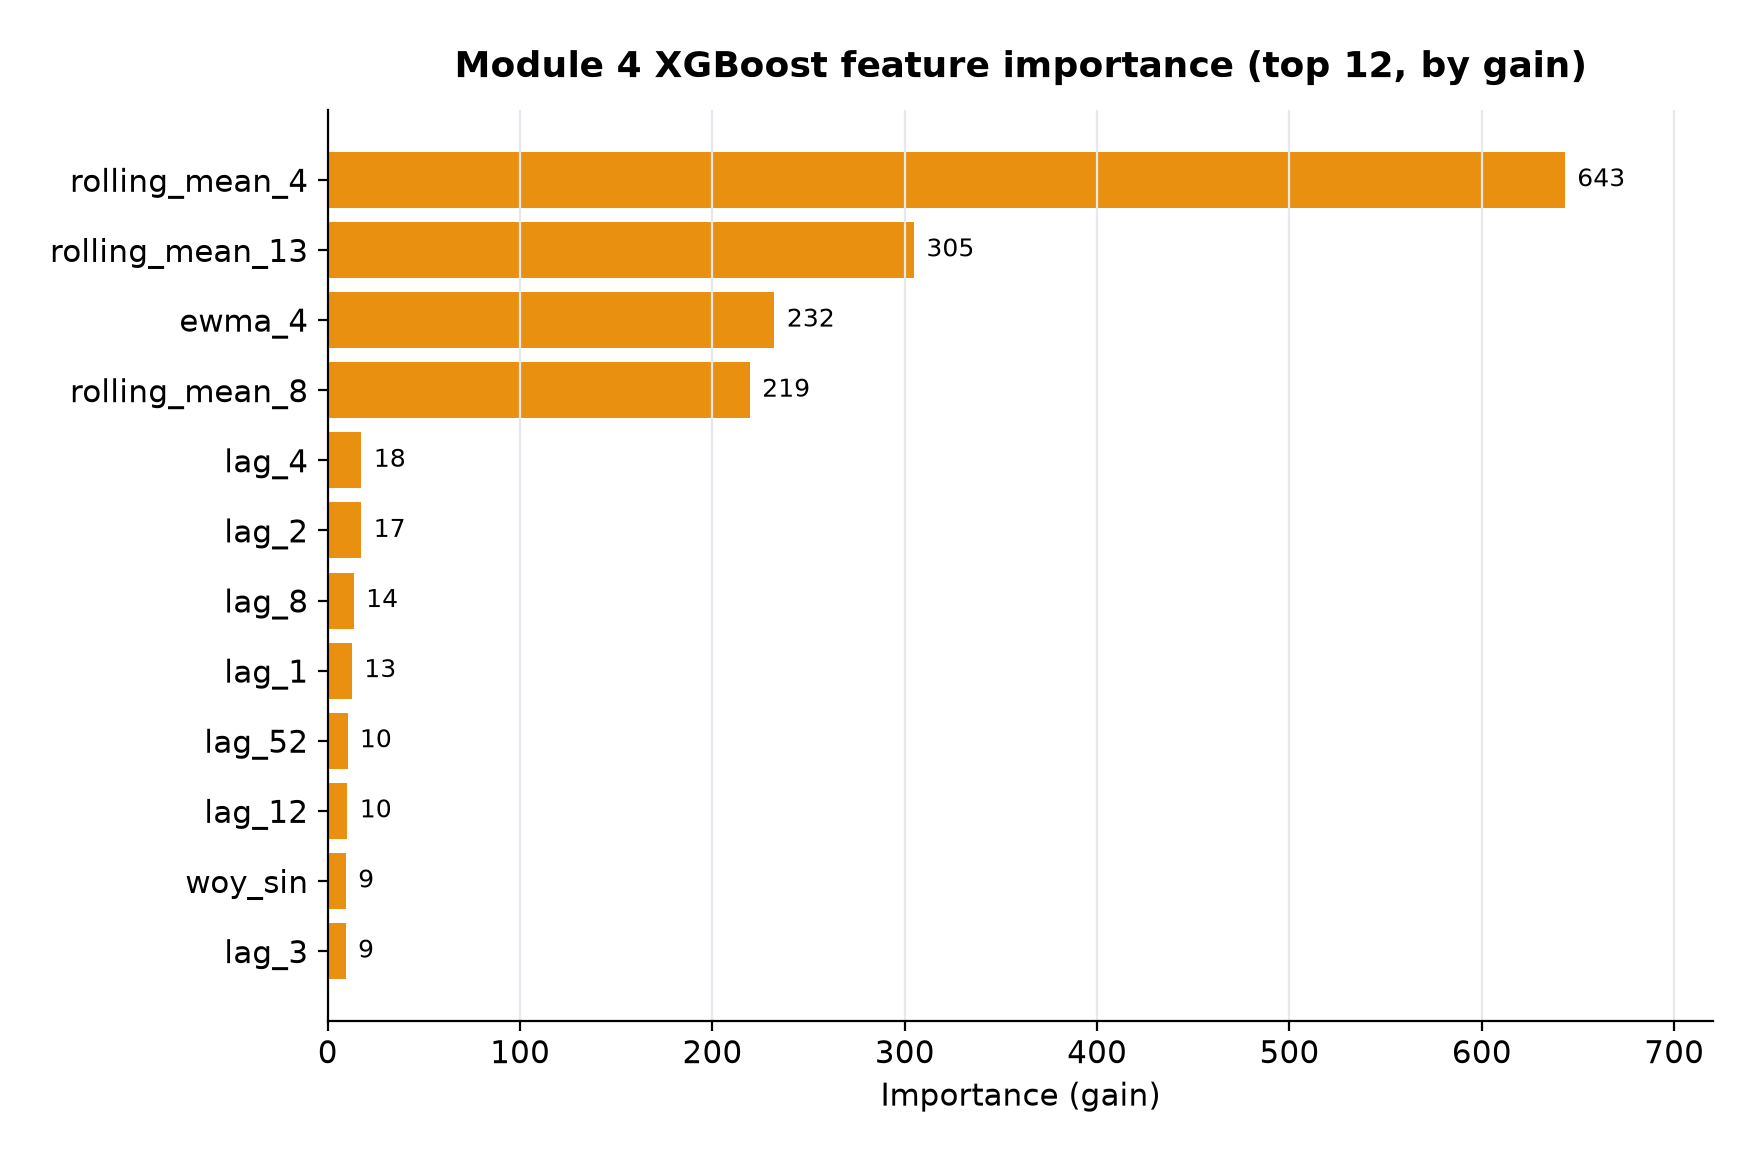
\includegraphics[width=0.82\textwidth]{fig13_m4_importance.png}
\caption{Module~4 XGBoost feature importance (top 12, by total gain). The short-window
rolling means (\texttt{rolling\_mean\_4/8/13}) and the exponentially weighted mean
dominate, far above the raw lags and calendar terms---demand is most predictable from
its own smoothed recent level, and the model has discovered this rather than relying on
the category identity we deliberately withheld.}
\label{fig:m4imp}
\end{figure}

%=============================================================================
\section{Discussion}

Put together, the results make one point: useful factory AI for small shops does
not need big models or the cloud. A 2.23~M detector matches a network ten times its
size and runs in milliseconds on a CPU, and boosted trees give sober maintenance and
demand numbers from modest tabular features. What we leaned on throughout was how the
models were tested --- separate splits, choices made on validation, baselines, and
repeated seeds --- because here a number that is too high is worse than one that is
merely good: it costs the owner the trust an alert depends on.

The maintenance result shows this most clearly. An $R^2$ of 0.545 looks plain next
to the vision accuracy, but it comes from the hardest fair test --- a tool the model
never saw --- and still doubles the linear baseline. The forecaster's edge over
Prophet is small in raw WAPE yet steady across folds, which is what a planner cares
about. These are numbers a shop can act on without a nasty surprise later.

The alert layer is simple, but it is not an afterthought. A model whose output the
operator cannot read helps no one on the floor. A fixed Hindi alert closes that gap
now and leaves room for a translation model later.

%=============================================================================
\section{Limitations}

We would rather state the edges of this work than gloss over them
(Table~\ref{tab:limits}). The big one: every number comes from public or synthetic
data, with no factory pilot, live sensor, or camera rig behind it. The casting task
separates easily, so its headline accuracy says little about harder defects. Some
baselines run on a single seed, a few defective parts still slip through, and the
maintenance and vision modules use different kinds of parts, so we have not shown
them working together on one physical line. The ROI figures that go with the
platform are editable targets, not measured results.

\begin{table}[H]
\caption{Limitations and honesty caveats.}
\label{tab:limits}
\centering
\small
\begin{tabular}{@{}cp{11.0cm}@{}}
\toprule
\# & Caveat \\
\midrule
L1 & Public/synthetic datasets only --- no factory pilot, live sensor, or camera rig. \\
L2 & Casting set is highly separable (a scratch CNN reaches $\approx99.4\%$); ceiling effect limits architecture claims. \\
L3 & Some baselines are single-seed; only the M1 architectures are run over three seeds. \\
L4 & Safety-critical false negatives (2--5 missed defects per seed) remain and are not yet cost-weighted. \\
L5 & M3 uses CNC-milled parts, not the castings of M1; the modules are not co-located on one line. \\
L6 & The demand dataset's final weeks are truncated (documented); figures trim this artifact, the model does not. \\
L7 & ROI figures are editable design-target projections, not measured deployment outcomes. \\
\bottomrule
\end{tabular}
\end{table}

%=============================================================================
\section{Conclusion and Future Work}

We built Drishti-AI, an offline system of four parts --- defect detection, a Hindi
alert, tool-wear prediction, and demand forecasting --- reporting to one dashboard
for a small manufacturer. On public data under a fair test, each part holds up:
99.4\% defect accuracy at 2.37~ms on a CPU, $R^2 = 0.545$ on unseen tools, and 19.7\%
WAPE that beats Prophet. It is a reproducible proof of concept, not a shipped
product.

The obvious next step is a real pilot --- wiring up one shop to test the parts on
its own castings, tools, and orders, and to measure the drop in scrap and downtime
we can only estimate here. After that: weight the defect threshold by cost to push
missed defects toward zero, widen the maintenance and forecasting baselines, and add
a neural Indic translator for richer operator guidance.

%=============================================================================
\begin{thebibliography}{99}
\small
\bibitem{sandler2018mobilenetv2} M. Sandler \emph{et al.}, ``MobileNetV2: Inverted Residuals and Linear Bottlenecks,'' \emph{CVPR}, 2018. \url{https://arxiv.org/abs/1801.04381}, doi:10.1109/CVPR.2018.00474.
\bibitem{howard2017mobilenets} A. Howard \emph{et al.}, ``MobileNets: Efficient CNNs for Mobile Vision,'' 2017. \url{https://arxiv.org/abs/1704.04861}.
\bibitem{he2016resnet} K. He \emph{et al.}, ``Deep Residual Learning for Image Recognition,'' \emph{CVPR}, 2016. doi:10.1109/CVPR.2016.90.
\bibitem{deng2009imagenet} J. Deng \emph{et al.}, ``ImageNet: A Large-Scale Hierarchical Image Database,'' \emph{CVPR}, 2009. doi:10.1109/CVPR.2009.5206848.
\bibitem{krizhevsky2012alexnet} A. Krizhevsky \emph{et al.}, ``ImageNet Classification with Deep CNNs,'' \emph{NeurIPS}, 2012. doi:10.1145/3065386.
\bibitem{simonyan2015vgg} K. Simonyan and A. Zisserman, ``Very Deep CNNs (VGG),'' \emph{ICLR}, 2015. \url{https://arxiv.org/abs/1409.1556}.
\bibitem{ioffe2015batchnorm} S. Ioffe and C. Szegedy, ``Batch Normalization,'' \emph{ICML}, 2015. \url{https://arxiv.org/abs/1502.03167}.
\bibitem{srivastava2014dropout} N. Srivastava \emph{et al.}, ``Dropout,'' \emph{JMLR}, 2014. \url{https://jmlr.org/papers/v15/srivastava14a.html}.
\bibitem{kingma2015adam} D. Kingma and J. Ba, ``Adam,'' \emph{ICLR}, 2015. \url{https://arxiv.org/abs/1412.6980}.
\bibitem{tan2019efficientnet} M. Tan and Q. Le, ``EfficientNet,'' \emph{ICML}, 2019. \url{https://arxiv.org/abs/1905.11946}.
\bibitem{chen2016xgboost} T. Chen and C. Guestrin, ``XGBoost: A Scalable Tree Boosting System,'' \emph{KDD}, 2016. doi:10.1145/2939672.2939785.
\bibitem{friedman2001gbm} J. Friedman, ``Greedy Function Approximation: A Gradient Boosting Machine,'' \emph{Ann. Statist.}, 2001. doi:10.1214/aos/1013203451.
\bibitem{breiman2001rf} L. Breiman, ``Random Forests,'' \emph{Machine Learning}, 2001. doi:10.1023/A:1010933404324.
\bibitem{ke2017lightgbm} G. Ke \emph{et al.}, ``LightGBM,'' \emph{NeurIPS}, 2017. \url{https://papers.nips.cc/paper/6907-lightgbm}.
\bibitem{lundberg2017shap} S. Lundberg and S.-I. Lee, ``A Unified Approach to Interpreting Model Predictions (SHAP),'' \emph{NeurIPS}, 2017. \url{https://arxiv.org/abs/1705.07874}.
\bibitem{pan2010transfer} S. J. Pan and Q. Yang, ``A Survey on Transfer Learning,'' \emph{IEEE TKDE}, 2010. doi:10.1109/TKDE.2009.191.
\bibitem{yosinski2014transferable} J. Yosinski \emph{et al.}, ``How Transferable Are Features in Deep Neural Networks?,'' \emph{NeurIPS}, 2014. \url{https://arxiv.org/abs/1411.1792}.
\bibitem{selvaraju2017gradcam} R. Selvaraju \emph{et al.}, ``Grad-CAM,'' \emph{ICCV}, 2017. doi:10.1109/ICCV.2017.74.
\bibitem{zhou2016cam} B. Zhou \emph{et al.}, ``Learning Deep Features for Discriminative Localization (CAM),'' \emph{CVPR}, 2016. \url{https://arxiv.org/abs/1512.04150}.
\bibitem{simonyan2013saliency} K. Simonyan \emph{et al.}, ``Deep Inside CNNs: Saliency Maps,'' 2013. \url{https://arxiv.org/abs/1312.6034}.
\bibitem{paszke2019pytorch} A. Paszke \emph{et al.}, ``PyTorch,'' \emph{NeurIPS}, 2019. \url{https://arxiv.org/abs/1912.01703}.
\bibitem{onnx} ONNX: Open Neural Network Exchange. \url{https://onnx.ai}.
\bibitem{onnxruntime} ONNX Runtime. \url{https://onnxruntime.ai}.
\bibitem{pedregosa2011sklearn} F. Pedregosa \emph{et al.}, ``Scikit-learn: Machine Learning in Python,'' \emph{JMLR}, 2011. \url{https://jmlr.org/papers/v12/pedregosa11a.html}.
\bibitem{harris2020numpy} C. Harris \emph{et al.}, ``Array Programming with NumPy,'' \emph{Nature}, 2020. doi:10.1038/s41586-020-2649-2.
\bibitem{mckinney2010pandas} W. McKinney, ``Data Structures for Statistical Computing in Python,'' \emph{SciPy}, 2010. doi:10.25080/Majora-92bf1922-00a.
\bibitem{hunter2007matplotlib} J. Hunter, ``Matplotlib: A 2D Graphics Environment,'' \emph{CiSE}, 2007. doi:10.1109/MCSE.2007.55.
\bibitem{jacob2018quantization} B. Jacob \emph{et al.}, ``Quantization for Efficient Integer-Arithmetic Inference,'' \emph{CVPR}, 2018. \url{https://arxiv.org/abs/1712.05877}.
\bibitem{hinton2015distill} G. Hinton \emph{et al.}, ``Distilling the Knowledge in a Neural Network,'' 2015. \url{https://arxiv.org/abs/1503.02531}.
\bibitem{warden2019tinyml} P. Warden and D. Situnayake, \emph{TinyML}, O'Reilly, 2019. \url{https://www.oreilly.com/library/view/tinyml/9781492052036/}.
\bibitem{taylor2018prophet} S. Taylor and B. Letham, ``Forecasting at Scale (Prophet),'' \emph{The American Statistician}, 2018. doi:10.1080/00031305.2017.1380080.
\bibitem{koenker1978quantile} R. Koenker and G. Bassett, ``Regression Quantiles,'' \emph{Econometrica}, 1978. doi:10.2307/1913643.
\bibitem{hyndman2021fpp} R. Hyndman and G. Athanasopoulos, \emph{Forecasting: Principles and Practice}, 3rd ed., 2021. \url{https://otexts.com/fpp3/}.
\bibitem{makridakis2020m4} S. Makridakis \emph{et al.}, ``The M4 Competition,'' \emph{Int. J. Forecasting}, 2020. doi:10.1016/j.ijforecast.2019.04.014.
\bibitem{hyndman2006accuracy} R. Hyndman and A. Koehler, ``Another Look at Measures of Forecast Accuracy,'' \emph{Int. J. Forecasting}, 2006. doi:10.1016/j.ijforecast.2006.03.001.
\bibitem{makridakis2022m5} S. Makridakis \emph{et al.}, ``The M5 Accuracy Competition,'' \emph{Int. J. Forecasting}, 2022. doi:10.1016/j.ijforecast.2021.11.013.
\bibitem{sokolova2009measures} M. Sokolova and G. Lapalme, ``A Systematic Analysis of Performance Measures for Classification,'' \emph{Inf. Proc. \& Mgmt}, 2009. doi:10.1016/j.ipm.2009.03.002.
\bibitem{saito2015prcurve} T. Saito and M. Rehmsmeier, ``The Precision-Recall Plot on Imbalanced Data,'' \emph{PLoS ONE}, 2015. doi:10.1371/journal.pone.0118432.
\bibitem{bouthillier2021variance} X. Bouthillier \emph{et al.}, ``Accounting for Variance in ML Benchmarks,'' \emph{MLSys}, 2021. \url{https://arxiv.org/abs/2103.03098}.
\bibitem{christ2018tsfresh} M. Christ \emph{et al.}, ``Time Series Feature Extraction (tsfresh),'' \emph{Neurocomputing}, 2018. doi:10.1016/j.neucom.2018.03.067.
\bibitem{dabhi2020casting} R. Dabhi, ``Casting Product Image Data for Quality Inspection,'' Kaggle. \url{https://www.kaggle.com/datasets/ravirajsinh45/real-life-industrial-dataset-of-casting-product}.
\bibitem{piecuch2025milling} Piecuch and Zabinski, ``CNC Milling Tool-Wear Dataset,'' 2025. \emph{[Confirm publisher/DOI record.]}
\bibitem{zhao2020demand} F. Zhao, ``Forecasts for Product Demand,'' Kaggle. \url{https://www.kaggle.com/datasets/felixzhao/productdemandforecasting}.
\bibitem{tabernik2020surface} D. Tabernik \emph{et al.}, ``Segmentation-Based Deep-Learning Approach for Surface-Defect Detection,'' \emph{J. Intell. Manuf.}, 2020. doi:10.1007/s10845-019-01476-x.
\bibitem{lei2018prognostics} Y. Lei \emph{et al.}, ``Machinery Health Prognostics: A Systematic Review,'' \emph{MSSP}, 2018. doi:10.1016/j.ymssp.2017.11.016.
\bibitem{zhao2019dlhealth} R. Zhao \emph{et al.}, ``Deep Learning for Machine Health Monitoring,'' \emph{MSSP}, 2019. doi:10.1016/j.ymssp.2018.05.050.
\bibitem{lee2015cps} J. Lee \emph{et al.}, ``A CPS Architecture for Industry 4.0 Manufacturing,'' \emph{Manufacturing Letters}, 2015. doi:10.1016/j.mfglet.2014.12.001.
\bibitem{kakwani2020indicnlp} D. Kakwani \emph{et al.}, ``IndicNLPSuite,'' \emph{Findings of EMNLP}, 2020. \url{https://aclanthology.org/2020.findings-emnlp.445/}.
\end{thebibliography}

\end{document}
